\chapter{Observational Scaling for Multi-Granular Long-Video Retrieval}
\label{ch:spatiotemporal-scaling}

\section{Introduction}

Chapter~\ref{ch:universal-video-retrieval} broadens the semantic conditions that a video representation is expected to support. Yet even a generalizable representation remains bounded by the visual evidence supplied to the model. This chapter therefore addresses observational scaling: how faithfully an embedding preserves the evidence required by queries at different temporal granularities under constrained sampling.

Real-world videos are increasingly long and informationally dense, spanning tens of minutes to hours~\cite{henschel2025streamingt2v,weng2024longvlm}, while a query may describe anything from the overall theme to a brief moment~\cite{xiao2022video,chen2023joint}. Since encoding every frame at full resolution is computationally prohibitive~\cite{hu2022mmsampler}, spatiotemporal sampling determines which evidence is available to the representation~\cite{guo2025gve}. Too few frames or too low a resolution can cause the target moment to be missed entirely. Although previous work has demonstrated sensitivity to sampling~\cite{guo2025gve,zhu2025dynamic}, its interaction with query granularity remains underexplored because no existing benchmark provides a multi-granular and controllable testbed. The relevant benchmark and embedding literature is reviewed centrally in \S\ref{sec:lr-benchmarks} and \S\ref{sec:lr-embedding}.

\begin{figure}[t]
    \centering
    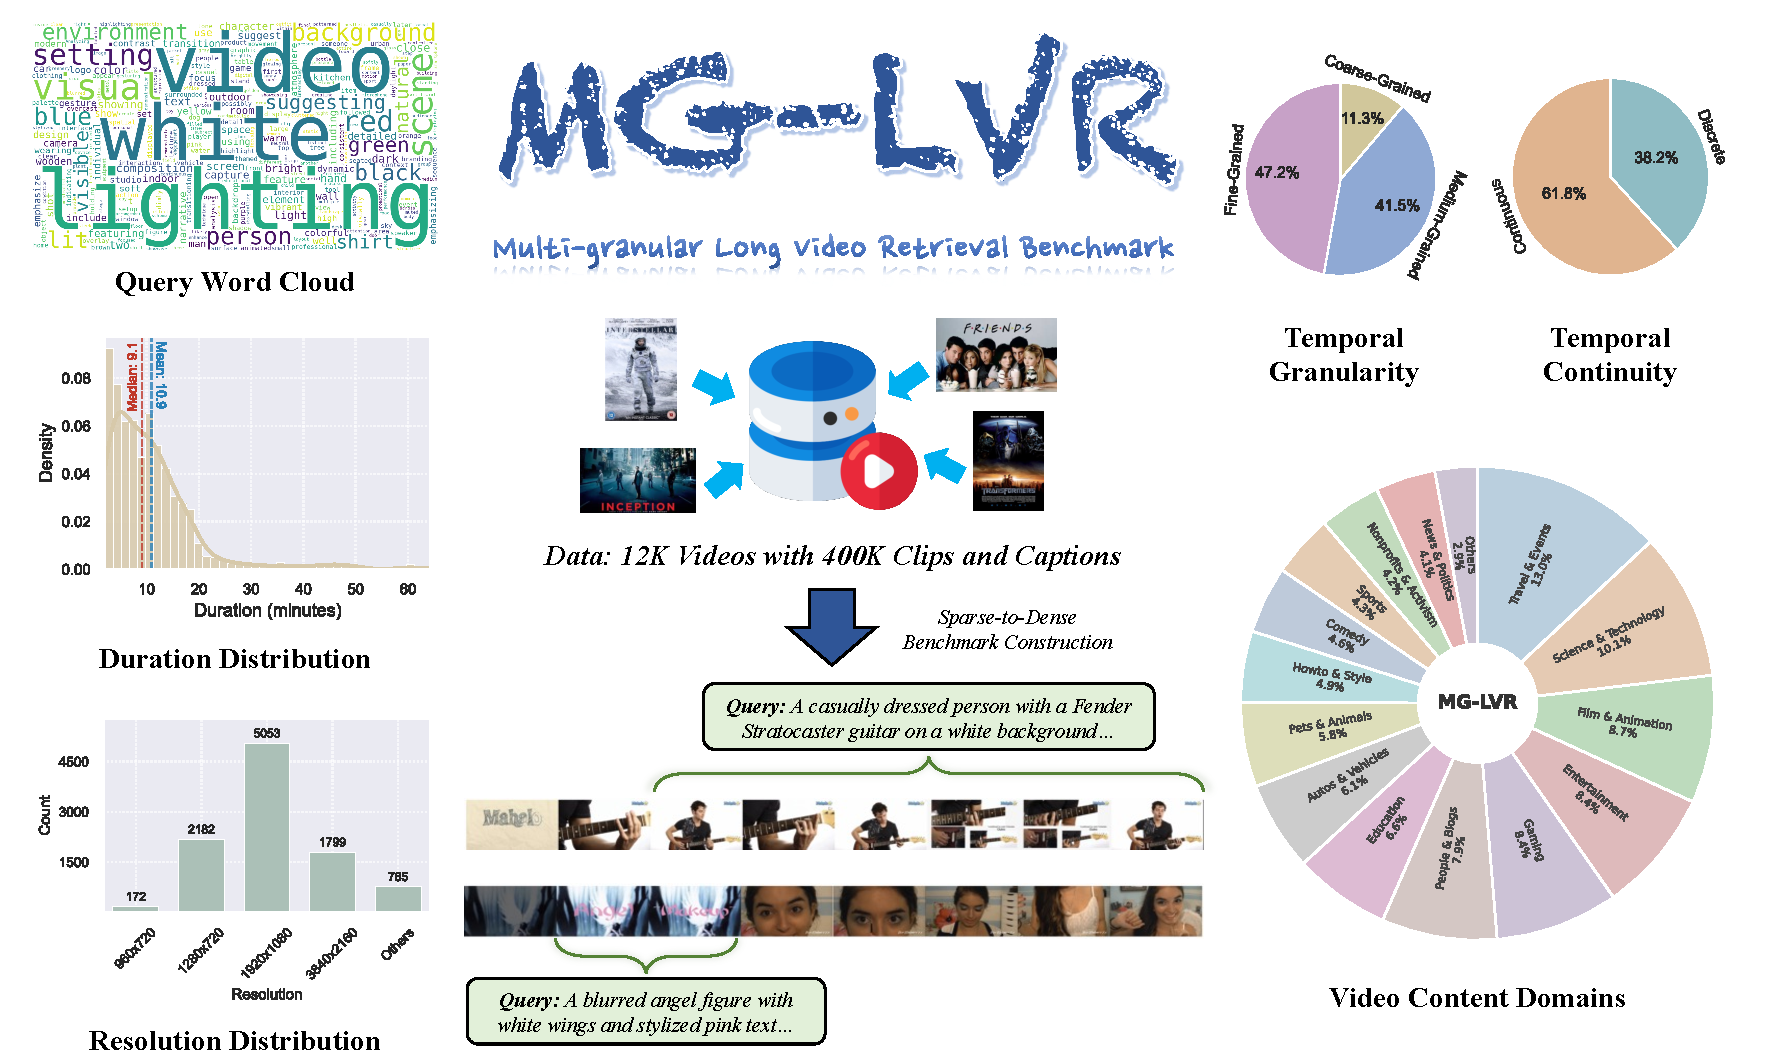
\includegraphics[width=\linewidth]{figures/mglvr/statistics.pdf}
    \caption{Overview of Multi-granular Long Video Retrieval (MG-LVR) benchmark.}
    \label{mglvr:fig:statistics}
\end{figure}

Current benchmarks are insufficient for this purpose. Short-clip datasets such as MSR-VTT~\cite{xu2016msr} and DiDeMo~\cite{anne2017localizing} are too brief for sampling density to have a meaningful impact. Recent long-video retrieval benchmarks~\cite{cai2025lovr} extend the temporal scope but evaluate at a single query granularity, making it impossible to determine whether sampling configurations should vary with query specificity. No existing setting jointly provides long-form videos and multi-granular query categorization within a unified evaluation framework. Such a combination is essential for exploring spatiotemporal scalability across diverse semantic scales.

To address this gap, we introduce the Multi-Granular Long Video Retrieval (\benchmarkname) benchmark shown in Figure~\ref{mglvr:fig:statistics}. \benchmarkname pairs long-form videos with queries categorized by temporal granularity, defined as the fraction of the video duration that a query covers. Importantly, the benchmark allows the relevant evidence for a query to be grounded either in a single clip or across multiple clips that may occur at different timestamps, reflecting realistic retrieval scenarios. Evaluation across 23 models reveals a pronounced granularity gap: fine-grained retrieval lags coarse-grained performance by over 75\% under sparse sampling and recovers only marginally as frame count increases. This provides a clear signal for studying how sampling configurations affect retrieval performance across different semantic granularities.

Using \benchmarkname, we conduct a comprehensive spatiotemporal scaling analysis across both Contrastive Language-Image Pretraining (CLIP)-based~\cite{gorti2022x} and Multimodal Large Language Model (MLLM)-based families~\cite{kong2025modality}. At test time, increasing spatial resolution helps most when frames are few, while its benefit saturates at higher frame counts. Under a fixed token budget, the optimal spatial-temporal allocation shifts with query granularity. Coarse queries favor fewer frames at higher resolution, while fine-grained queries favor more frames at lower resolution. At training time, the interaction between spatial and temporal density is asymmetric. Spatial representations are resolution-robust, maintaining accuracy across varying input resolutions. Temporal representations exhibit frame-count anchoring, where performance peaks when the inference frame count matches the training configuration and degrades significantly when they diverge, particularly for fine-grained queries.

This analysis highlights a key insight: the knowledge required for effective low-density inference is already latent within high-density models, but it does not automatically transfer when the sampling configuration changes. To address this, we propose Video Embedding Waterfall (VEterfall), a progressive dense-to-sparse self-distillation framework. Inspired by the waterfall effect, our method cascades high-fidelity semantic knowledge from densely sampled embeddings down to sparser representations. In this way, VEterfall achieves up to a 20\% relative recall gain on fine-grained queries while operating in a 4$\times$ to 16$\times$ more efficient inference setting. Our experiments confirm that the scaling behaviors identified by \benchmarkname can be directly and effectively exploited in practice.

The contributions of this chapter are summarized as follows.
(1)~We introduce \benchmarkname, the first benchmark for multi-granular long-video retrieval that enables scalable research into spatiotemporal sampling.
(2)~We conduct a multi-dimensional scaling analysis that identifies key principles such as frame-count anchoring and granularity-dependent token allocation.
(3)~We propose VEterfall, a self-distillation method that enhances video embeddings under sparse sampling by unlocking multi-granular knowledge already latent within the models.


\begin{table}[t]
    \centering
    \caption{Comparison of text-video retrieval benchmarks. \textbf{MG-LVR} is the first benchmark supporting multi-granular queries for retrieving long-form videos. \textbf{Gran.}: Temporal granularity of queries, including fine~(FN), medium~(MD), and coarse~(CR) -grained; \textbf{Cont.}: Temporal continuity of queries, including discrete~(DC) and continuous~(CT).}
    \label{mglvr:tab:benchmark_comparison}
    \setlength{\tabcolsep}{2.5pt}
    \begin{tabular}{@{}l*{6}{c}@{}}
    \toprule
    \textbf{Dataset} & \textbf{\#~Query} & \textbf{\#~Corpus} & \textbf{Dur~(s)} & \textbf{\#~Word} & \textbf{Gran.} & \textbf{Cont.} \\
    \midrule
    MSRVTT~\cite{xu2016msr} & 1,000 & 1,000 & 15.0 & 9.4 & CR & CT \\
    DiDeMo~\cite{anne2017localizing} & 1,004 & 1,004 & 53.9 & 29.1 & CR & CT \\
    TVR~\cite{lei2020tvr} & 10,895 & 2,179 & 76.2 & 13.4 & FN, MD & CT \\
    ActivityNet Captions~\cite{krishna2017dense} & 18,000 & 4,917 & 117.6 & 14.8 & FN, MD & CT \\
    LoVR~\cite{cai2025lovr} & 100 & 467 & 1560.3 & 17364.5 & CR & CT \\
    VDC~\cite{chai2024auroracap} & 1,000 & 1,027 & 30.1 & 508.0 & CR & CT \\
    \midrule
    \textbf{MG-LVR (Ours)} & 9,971 & 4,844 & 705.9 & 44.7 & All & Both \\
    \bottomrule
    \end{tabular}
\end{table}

\section{Rethinking Text-Video Retrieval Evaluation}
\label{mglvr:sec:benchmark}

Text-video retrieval has historically been formulated as a global-matching task, where each query describes the entirety of its paired video. This convention reflects the structural limitations of existing benchmarks: queries are either brief summaries of short clips or document-level aggregations of dense captions, making the query and video co-extensive by construction and effectively sidestepping the challenge of temporal scale. In the era of long, multi-scene video, this paradigm is insufficient. User intent may range from identifying a moment of a few seconds within an hour-long lecture to capturing the overarching theme of an entire documentary, imposing qualitatively different demands on spatiotemporal sampling and representation density.

As shown in Figure~\ref{mglvr:fig:statistics}, the \textbf{Multi-Granular Long Video Retrieval (MG-LVR)} benchmark is designed to bridge this gap by formalizing \textit{temporal granularity} as an explicit evaluation axis. Unlike traditional datasets~\cite{lei2020tvr,krishna2017dense} where granularity emerges as a byproduct of annotator bias and video readability~(e.g., length, dynamics, complexity), \benchmarkname employs an automated pipeline that explicitly controls query granularity by analyzing semantic relationships among clips within each video, enabling a systematic study of how models navigate the spectrum from localized events to global narratives. The resulting benchmark contains $9,971$ queries paired with a corpus of $4,844$ videos averaging $705.9$ seconds in duration. As summarized in Table~\ref{mglvr:tab:benchmark_comparison}, \benchmarkname is the only benchmark that jointly covers all three granularity levels while supporting both single-clip and multi-clip evidence structures. The dataset and code of MG-LVR will be publicly released upon acceptance. This section first formalizes the evaluation setting, then describes the construction pipeline, and concludes with the complete prompt specifications used for query and caption synthesis.

\subsection{Formulations}
\label{mglvr:sec:formulation}

This chapter retains the query $q$, corpus $\mathcal{V}$, and ranking objective from the unified formulation in \S\ref{sec:bc-vr}. It specializes that formulation to text queries over long-form videos and introduces temporal granularity as an observational variable rather than a different retrieval objective.

Accordingly, the target is $v^{*} = \arg\max_{v \in \mathcal{V}} s(q,v)$. The query may refer to any portion of the video, from a brief localized event to the overall theme, with the fraction of relevant content serving as a variable difficulty factor.

\begin{definition}[\textbf{Temporal Granularity}]
Temporal granularity $G$ is defined as the ratio of relevant content duration to total video length:
\begin{equation}
    G = \frac{|\mathcal{S}(v^{*},\,q)|}{d_{\mathrm{video}}} \in (0,\,1].
    \label{mglvr:eq:granularity}
\end{equation}
As $G \to 0$, retrieval approaches a needle-in-a-video problem in which the target moment occupies a vanishingly small fraction of the video. For systematic evaluation, we partition the granularity spectrum into three categories: \textbf{Fine-grained (FN)}, \textbf{Medium-grained (MD)}, and \textbf{Coarse-grained (CR)}.
\end{definition}

In this work, granularity thresholds are set to $G \in [0.001, 0.01]$ for FN and $G \in [0.1, 0.3]$ for MD, ensuring high inter-class distinctiveness and enabling clear observation of how model performance scales with task difficulty.

For the temporal distribution of relevant content, we further define temporal continuity $C$ to characterize the structural complexity of each retrieval target:
\begin{equation}
    C = \frac{\sum_{i=1}^{k}(e_i - s_i)}{e_k - s_1} \in (0,\,1],
    \label{mglvr:eq:continuity}
\end{equation}
where $[s_i, e_i]$ are the $k$ disjoint intervals composing $\mathcal{S}$. A value of $C=1$ indicates a single contiguous event, while $C<1$ represents fragmented content distributed across multiple disjoint segments, such as a recurring theme.

\begin{figure}[t]
    \centering
    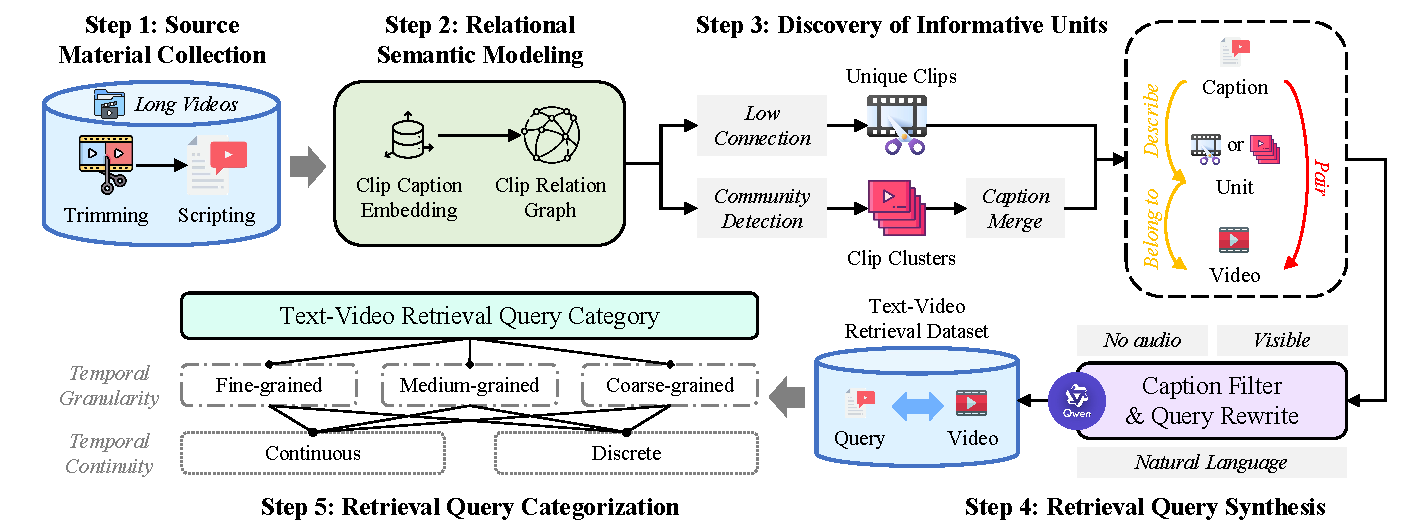
\includegraphics[width=\linewidth]{figures/mglvr/mg-lvr.pdf}
    \caption{The \benchmarkname construction pipeline. We model long videos as \textit{Clip Relation Graphs} to transform unstructured content into a quantifiable semantic topology. This structural foundation allows for the systematic discovery of retrieval units across varying temporal granularities and continuity levels, which are then synthesized by an LLM into natural language queries.}
    \label{mglvr:fig:mg-lvr}
\end{figure}

\subsection{MG-LVR: Sparse-to-Dense Benchmark Construction}
\label{mglvr:sec:construction}

As summarized in Figure~\ref{mglvr:fig:mg-lvr}, we construct \benchmarkname through a semantics-aware pipeline that formalizes video retrieval as a sampling task over structured semantic relationships among clips. The core insight is to represent each video as a similarity graph, enabling the identification of retrieval units that vary in temporal granularity and evidence composition. This approach ensures that \benchmarkname covers scenarios where relevant evidence is grounded either in a single clip or across multiple clips that may occur at different timestamps.

\paragraph{Step 1: Material Curation.}
We build upon the Vript dataset~\cite{yang2024vript}, selecting long videos ($>120$s) with dense, high-quality GPT-4V clip-level captions. These captions serve as semantic proxies, allowing the pipeline to model video content without the prohibitive cost of pixel-level processing during construction.

\paragraph{Step 2: Semantic Topology Modeling.}
To provide a structural basis for unit extraction, each video is represented as a \textit{Clip Relation Graph}, where nodes correspond to clips, and edges correspond to the cosine similarity values between two clip caption embeddings produced by Qwen3-Embedding-8B~\cite{qwen3embedding}. This graph captures semantic relationships among clips: clusters of highly connected nodes often correspond to dominant themes, while weaker connections may indicate localized or transient events.

\paragraph{Step 3: Discovery of Informative Units.}
Retrieval units are extracted from the clip relation graph by applying structural constraints that correspond to our granularity and evidence composition settings. This graph-based discovery allows the benchmark to include both single-clip evidence and semantically related clips that appear at different timestamps.
\textit{Single-Clip Units:} Individual nodes with nearly zero external connections are selected as standalone retrieval units, yielding $32,984$ units.
\textit{Multi-Clip Units:} Identified via Louvain community detection to capture thematically consistent clips that may be dispersed across the timeline, yielding $7,764$ units.

\paragraph{Step 4: Retrieval Query Synthesis.}
An LLM (Qwen3-32B~\cite{yang2025qwen3}) synthesizes the metadata of each unit into a natural language query. For multi-clip units, the model is prompted to generate a holistic description covering the relationships among multiple relevant clips. A subsequent refinement pass filters out ambiguous descriptions and removes references to audio content to ensure a focus on visual information.

\paragraph{Step 5: Retrieval Query Categorization.}
Each query-video pair is assigned to a granularity level (FN, MD, or CR) based on the computed value of $G$. The final benchmark retains $9,971$ queries in total, comprising $4,706$, $4,142$, and $1,123$ queries for FN, MD, and CR, respectively.

\paragraph{Human Validation.}
To ensure retrieval uniqueness, a cross-modal collision check is applied: queries exhibiting high semantic similarity to non-target clips within the same video are pruned. Human validation confirms a $96\%$ accuracy rate over $50$ query-video pairs.


\subsection{Prompt Specifications for MG-LVR Construction}
\label{mglvr:sec:prompt_specs}
% ============================================================

Step~4 of the MG-LVR construction pipeline uses two LLM prompts: one generates retrieval queries from clip-level captions (\S\ref{mglvr:sec:prompt_query}), and the other synthesizes a consolidated visual description of each video (\S\ref{mglvr:sec:prompt_caption}). Both prompts were executed with Qwen3-32B.

\subsubsection{Retrieval Query Synthesis}
\label{mglvr:sec:prompt_query}

This prompt is used in Step~4. It receives the aggregated captions of a retrieval unit together with its granularity $G$ and continuity $C$ values, and produces three natural-language queries of increasing descriptive depth.

\begin{promptbox}{Retrieval Query Synthesis from Captions}
\begin{lstlisting}[style=promptstyle]
## ROLE
You are an expert Search Query Synthesizer. Your primary goal is to read a descriptive video caption and generate three high-quality, divergent search queries that are strictly grounded in the visual information provided.

## CRITICAL RULES & PROCESSING LOGIC

### 1. Core Mandate: Grounded and Diverse Queries
- **Strictly Visual & Factual**: All generated queries, regardless of their complexity, MUST be derived solely from the visual information described in the "Raw Caption". Do not invent details not present (e.g., specific brand names unless visible, people's names unless specified as visual text). Explicitly ignore any mention of audio, speech, voice-overs, sound effects, or metadata. Queries must be declarative sentences, not questions or commands.
- **Three Distinct Perspectives**: For each valid caption, generate exactly three queries. These queries must be genuinely different, reflecting diverse user intents and levels of detail.
  - **Query 1 (Librarian/Factual)**: A concise, objective summary of the core visual elements. Length: 20-50 words.
  - **Query 2 (Everyday User/Descriptive)**: A more narrative and descriptive query, using richer vocabulary to describe the scene, actions, and atmosphere. Length: 30-100 words.
  - **Query 3 (Researcher/Analytical)**: A detailed, analytical query that examines visual composition, spatial-temporal details, potential technical aspects, or the narrative storytelling of the scene. Length: 70-200 words.

### 2. Content Quality Filter: Identify and Discard Invalid Inputs
- Before generating queries, you MUST first assess the "Raw Caption" against the following filters. If a caption falls into any of these categories, you MUST return an empty list `[]` for "refined_queries".
- **A clip is considered INVALID if its caption describes:**
  1.  **No Visual Content**: An entirely blank, black, white, or single-color screen with no other discernible objects, text, or shapes.
  2.  **Irretrievably Low Quality**: Content that is explicitly stated to be too blurry, corrupted, pixelated, or overexposed to identify any subjects, objects, or actions.
  3.  **Purely Abstract/Non-Representational**: Content consisting only of abstract patterns, fractals, kaleidoscope effects, or color fields without any concrete, recognizable subjects. (e.g., "a swirling vortex of psychedelic colors").
  4.  **Extremely Low Information Density**: A single, simple, static, or looping scene with minimal change over a long duration, making the generation of three diverse, meaningful queries impossible. (e.g., "a 10-minute video of a spinning fan" or "a static image of a single apple on a table").
  5.  **Dense Text/Code as Primary Content**: Screen recordings that primarily show large, scrolling blocks of code, documents, or dense text where the main subject is the textual information itself, not a visual narrative or action. (This does not apply to simple title cards or logos).
  6.  **Refusals or Error Messages**: The caption is an apology, a refusal to describe (e.g., "I'm sorry, I cannot describe..."), or an error message.

### 3. Special Handling for Minimalist Content
- If the caption describes a very simple scene (e.g., a plain background) but **also contains a key visual element** like a logo, a title card, or a single piece of text (e.g., 'LATINO' on a black screen), it is considered **VALID**.
- In such cases, your queries must **focus intently on these minimal elements**. Describe their visual properties (font, color, style, placement) and, for the researcher query, analyze their likely function (e.g., branding, title sequence, call-to-action).

## OUTPUT FORMAT
You MUST return ONLY a single, strict JSON object. No explanations or conversational text. The required format is:
{"refined_queries": ["Librarian query text", "Everyday user query text", "Researcher query text"]}

- If the input is deemed invalid based on the "Content Quality Filter", the output MUST be:
{"refined_queries": []}

**Metadata**: Granularity={granularity}, Continuity={continuity}
**Raw Caption**: {caption}

**JSON Output**:
\end{lstlisting}
\end{promptbox}

\subsubsection{Clip Caption Merging}
\label{mglvr:sec:prompt_caption}

This prompt produces a consolidated visual-only description of each video from its clip-level captions. The output serves as the semantic proxy for building the Clip Relation Graph ($\mathcal{G}$) in Step~2, and is also used during the refinement pass in Step~4 to filter out queries that reference non-visual content.

\begin{promptbox}{Clip Caption Merging in Groups}
\begin{lstlisting}[style=promptstyle]
## Role & Core Principle
You are a master video summarizer, operating as a **Visual Purist**. Your absolute primary goal is to create a single, flowing paragraph that describes only what a person would see if they watched the video with the sound completely off.

**Your Most Important Rule: Proactive Filtering.**
You MUST critically analyze the input `caption` for each clip and proactively filter out any information that is not strictly visual. **Completely ignore and do not mention**:
-   **Spoken Content**: Dialogue, narration, interviews, or any transcribed speech (e.g., "the narrator explains...", "discusses the importance of...").
-   **Character/Object Names & Backstories**: Proper names of people, places, or things (e.g., "Midas the mouse," "the Napa fires"), unless they are clearly visible as text in the scene (e.g., a brand name on a product).
-   **Abstract Concepts & Inferred Knowledge**: Intentions, emotions, technical jargon (e.g., "'Inverted Single Stroke Four' drum fill"), or specialized knowledge that cannot be seen directly (e.g., "the car's engine is powerful").
-   **Audio Cues**: Descriptions of music, sound effects, or tone of voice.

## Input Analysis & Synthesis Logic
Follow this structured three-step process to generate the summary:

**Step 1: Identify the Core Subject & Setting.**
-   Quickly scan all clip captions to determine the recurring central subject (e.g., a person, an animal, an object) and the primary environment (e.g., a kitchen, a forest, a studio). This forms the foundation of your summary.

**Step 2: Construct the Narrative Flow.**
-   Start your summary by introducing the core subject and setting you identified.
-   Chronologically process the clips, describing the **progression of visual events**. Use temporal cues like "The video begins with...", "As the demonstration progresses...", "Later, the scene shifts to...", and "The video concludes by showing..." to create a coherent narrative.
-   Give more descriptive weight to clips with a higher `temporal_ratio`, as they represent more of the video's runtime.
-   **Crucially**, also integrate unique, visually striking details from shorter clips, especially if they show a distinct action, a close-up of a key object, or a significant change in the scene. This ensures the summary is both representative and rich in detail.

**Step 3: Refine and Polish.**
-   Ensure the final text is a single, well-written paragraph.
-   Read through your summary one last time to confirm it is 100 percent based on visual information and flows logically from beginning to end.

## Handling Inconsistencies & Corner Cases
-   **Conflicting Visuals**: If clips describe conflicting details (e.g., wall color changes from 'purple' to 'beige'), either describe the most dominant/frequently-seen version or briefly acknowledge the change (e.g., "...in a room with walls that appear alternately purple and beige."). **Do not** create an inaccurate hybrid description.
-   **Invalid/Empty Clips**: If a clip's caption is an error message, a refusal, or contains no visual information, ignore it completely.

## Output Specification
-   Your output MUST be ONLY a single, valid JSON object.
-   The JSON object must have two keys: `video_id` (string) and `caption` (string).
-   The `caption` should be a single paragraph, typically between 30 and 200 words.

## Input
Video ID: {video_id}
Clips (clip_id | caption | span | ratio):
{clips}
\\

\#\# Output:
\end{lstlisting}
\end{promptbox}

\FloatBarrier
\section{Spatiotemporal Scaling Laws: Experiments, Analysis, and Discoveries}
\label{mglvr:sec:scaling}

Leveraging \benchmarkname as a controlled testbed, we systematically analyze how spatiotemporal sampling density affects retrieval performance across query granularity levels. The analysis proceeds in four phases. We first compare baselines under default configurations. We then study test-time scaling by varying spatial and temporal densities during inference, followed by training-time scaling to examine how the training density affects the learned embeddings. Finally, case studies illustrate representative limitations behind the aggregate results.

\subsection{Experimental Setup}

\paragraph{Model Selection.}
Twenty-three models from two paradigms are evaluated: 6 CLIP-based models and 17 MLLM-based models.

\begingroup\emergencystretch=2em
CLIP-based models:
CLIP4Clip~\cite{luo2022clip4clip} (87M);
ViCLIP~\cite{wang2023internvid} (0.4B);
VideoCLIP-XL~\cite{wang2024videoclip} (0.4B);
LanguageBind-Video-Huge-V1.5~\cite{zhu2024languagebind} (1.2B);
InternVideo2-Stage2-1B~\cite{wang2024internvideo2} (1.4B);
InternVideo2-Stage2-6B~\cite{wang2024internvideo2} (6.4B).

MLLM-based models:
gme-Qwen2-VL-2B-Instruct~\cite{Zhang_2025_CVPR} (GME-2B, 2.2B);
Unite-Base-Qwen2-VL-2B~\cite{kong2025modality} (Unite-2B, 2.2B);
VLM2Vec-V2.0~\cite{meng2025vlm2vec} (VLM2Vec-V2, 2.2B);
Ops-MM-embedding-v1-2B~\cite{ops} (Ops-MM-2B, 2.2B);
GVE-3B~\cite{guo2025gve} (GVE-3B, 3.8B);
Qwen3-VL-Embedding-2B~\cite{qwen3vlembedding} (Qwen3-VL-Emb-2B, 2.1B);
BGE-VL-v1.5-mmeb~\cite{zhou2024megapairs} (BGE-VL, 7.6B);
UniME-V2-LLaVA-OneVision-8B~\cite{gu2025unime} (UniME-V2, 8.0B);
B3-Qwen2-7B~\cite{thirukovalluru2025breaking} (B3-7B, 8.3B);
gme-Qwen2-VL-7B-Instruct~\cite{Zhang_2025_CVPR} (GME-7B, 8.3B);
Unite-Base-Qwen2-VL-7B~\cite{kong2025modality} (Unite-7B, 8.3B);
Ops-MM-embedding-v1-7B~\cite{ops} (Ops-MM-7B, 8.3B);
U-MARVEL-Qwen2VL-7B-Instruct~\cite{li2026umarvel} (U-MARVEL, 8.3B);
LamRA-Ret-Qwen2.5VL-7B~\cite{liu2025lamra} (LamRA-Ret, 8.3B);
GVE-7B~\cite{guo2025gve} (GVE-7B, 8.3B);
RzenEmbed-7B~\cite{jian2025rzenembed} (RzenEmbed, 8.3B);
Qwen3-VL-Embedding-8B~\cite{qwen3vlembedding} (Qwen3-VL-Emb-8B, 8.1B).
\par\endgroup

\paragraph{Evaluation Protocol.}
Retrieval performance is measured using Recall@1 (R@1) and Mean Reciprocal Rank (MRR) across three query granularity levels: Fine-grained (FN), Medium-grained (MD), and Coarse-grained (CR). The total visual token budget per video is defined as $N_{\text{total}} = F \times T$, where $F$ denotes the number of uniformly sampled frames and $T$ denotes the number of spatial tokens per frame as determined by the visual encoder. In the analyses that follow, $F$ and $T$ are varied independently while all other experimental factors are held constant to isolate the effect of sampling density.

\subsection{Baseline Comparison}
\label{mglvr:sec:baseline}

Tables~\ref{mglvr:tab:main_results_8f}, \ref{mglvr:tab:main_results_32f}, and~\ref{mglvr:tab:main_results_128f} present the available results at 8, 32, and 128 frames in increasing order. The 8-frame comparison covers all twenty-three models, while the larger-budget tables report the models evaluated at those settings. Performance degrades consistently from CR to FN across the reported architectures, regardless of model family, parameter scale, or training data composition. For Qwen3-VL-Emb-8B, R@1 drops from $0.8557$ on CR to $0.2102$ on FN at 8 frames, a relative decline of over 75\%. At 32 frames, the corresponding FN score rises to $0.2641$, while the CR score rises to $0.8976$. Even at 128 frames, FN R@1 improves only modestly to $0.2871$, a gain of less than 8 percentage points over the 8-frame result despite a $16\times$ increase in temporal sampling density. This pronounced granularity gradient indicates that additional frames improve temporal coverage but yield strongly diminishing returns on fine-grained retrieval.

\begin{table}[t]
    \centering
    \caption{Multi-granularity retrieval performance of all baselines at 8 uniformly sampled frames per video. Bold and underline indicate the best and second-best results within each model group, respectively.}
    \label{mglvr:tab:main_results_8f}
    \setlength{\tabcolsep}{2pt}
    \begin{tabular}{@{}l*{8}{c}@{}}
\toprule
Model & \multicolumn{2}{c|}{Overall} & \multicolumn{2}{c|}{FN} & \multicolumn{2}{c|}{MD} & \multicolumn{2}{c}{CR} \\
      & R@1   & MRR   & R@1   & MRR   & R@1   & MRR   & R@1   & MRR \\
\midrule
InternVideo2-1B         & 0.2398 & 0.3216 & 0.0803 & 0.1383 & 0.3390 & 0.4435 & 0.5423 & 0.6398 \\
ViCLIP                  & 0.2659 & 0.3491 & 0.1054 & 0.1714 & 0.3790 & 0.4772 & 0.5209 & 0.6207 \\
CLIP4Clip               & 0.2696 & 0.3561 & 0.1067 & 0.1703 & 0.3660 & 0.4757 & 0.5966 & 0.6938 \\
InternVideo2-6B         & 0.2890 & 0.3757 & 0.1069 & 0.1756 & 0.4029 & 0.5093 & 0.6322 & 0.7215 \\
VideoCLIP-XL            & \underline{0.3914} & \underline{0.4794} & \underline{0.1687} & \underline{0.2488} & \underline{0.5449} & \underline{0.6466} & \textbf{0.7587} & \textbf{0.8293} \\
LanguageBind            & \textbf{0.4194} & \textbf{0.5046} & \textbf{0.1997} & \textbf{0.2811} & \textbf{0.5787} & \textbf{0.6728} & \underline{0.7524} & \underline{0.8204} \\
\midrule
GME-2B                  & 0.2793 & 0.3642 & 0.1128 & 0.1783 & 0.3754 & 0.4816 & 0.6224 & 0.7101 \\
Unite-2B                & 0.2875 & 0.3728 & 0.1169 & 0.1834 & 0.3889 & 0.4936 & 0.6287 & 0.7213 \\
Ops-MM-2B               & 0.3085 & 0.3893 & 0.1258 & 0.1918 & 0.4211 & 0.5180 & 0.6589 & 0.7416 \\
VLM2Vec-V2              & 0.3089 & 0.3870 & 0.1243 & 0.1833 & 0.4162 & 0.5147 & 0.6866 & 0.7695 \\
GVE-3B                  & \underline{0.3747} & \underline{0.4593} & \underline{0.1583} & \underline{0.2358} & \underline{0.5128} & \underline{0.6100} & \textbf{0.7720} & \textbf{0.8397} \\
Qwen3-VL-Emb-2B         & \textbf{0.3914} & \textbf{0.4751} & \textbf{0.1723} & \textbf{0.2481} & \textbf{0.5386} & \textbf{0.6348} & \underline{0.7667} & \underline{0.8375} \\
\midrule
U-MARVEL                & 0.1169 & 0.1919 & 0.0368 & 0.0784 & 0.1526 & 0.2501 & 0.3215 & 0.4528 \\
LamRA-Ret               & 0.1885 & 0.2671 & 0.0858 & 0.1414 & 0.2566 & 0.3516 & 0.3678 & 0.4822 \\
GME-7B                  & 0.3161 & 0.4018 & 0.1309 & 0.2004 & 0.4278 & 0.5326 & 0.6803 & 0.7630 \\
BGE-VL                  & 0.3201 & 0.4000 & 0.1362 & 0.2018 & 0.4425 & 0.5376 & 0.6394 & 0.7228 \\
B3-7B                   & 0.3475 & 0.4282 & 0.1519 & 0.2211 & 0.4657 & 0.5627 & 0.7311 & 0.7999 \\
Ops-MM-7B               & 0.3546 & 0.4357 & 0.1538 & 0.2258 & 0.4778 & 0.5733 & 0.7418 & 0.8076 \\
RzenEmbed               & 0.3707 & 0.4541 & 0.1498 & 0.2246 & 0.5118 & 0.6101 & 0.7756 & 0.8402 \\
Unite-7B                & 0.3733 & 0.4591 & 0.1664 & 0.2453 & 0.5007 & 0.6011 & 0.7703 & 0.8312 \\
UniME-V2                & 0.3881 & 0.4721 & 0.1575 & 0.2338 & 0.5447 & 0.6415 & 0.7774 & 0.8458 \\
GVE-7B                  & \underline{0.4121} & \underline{0.4960} & \underline{0.1813} & \underline{0.2634} & \underline{0.5652} & \underline{0.6590} & \underline{0.8148} & \underline{0.8693} \\
Qwen3-VL-Emb-8B         & \textbf{0.4492} & \textbf{0.5269} & \textbf{0.2102} & \textbf{0.2861} & \textbf{0.6106} & \textbf{0.6993} & \textbf{0.8557} & \textbf{0.9002} \\
\bottomrule
\end{tabular}
\end{table}

\begin{table}[t]
\centering
\caption{Multi-granularity retrieval performance of the baselines evaluated at 32 uniformly sampled frames per video. Bold and underline indicate the best and second-best results within each model group, respectively.}
\label{mglvr:tab:main_results_32f}
\setlength{\tabcolsep}{2pt}
\begin{tabular}{@{}l|*{8}{c}@{}}
\toprule
Model & \multicolumn{2}{c|}{Overall} & \multicolumn{2}{c|}{FN} & \multicolumn{2}{c|}{MD} & \multicolumn{2}{c}{CR} \\
      & R@1 & MRR & R@1 & MRR & R@1 & MRR & R@1 & MRR \\
\midrule
InternVideo2-1B  & 0.1948 & 0.2653 & 0.0463 & 0.0890 & 0.2641 & 0.3611 & 0.5610 & 0.6512 \\
InternVideo2-6B  & 0.2815 & 0.3674 & 0.0963 & 0.1620 & 0.3940 & 0.5022 & \underline{0.6429} & \underline{0.7305} \\
CLIP4Clip        & \underline{0.3087} & \underline{0.3955} & \underline{0.1220} & \underline{0.1924} & \underline{0.4302} & \underline{0.5360} & \underline{0.6429} & 0.7286 \\
LanguageBind     & \textbf{0.4622} & \textbf{0.5445} & \textbf{0.2284} & \textbf{0.3153} & \textbf{0.6374} & \textbf{0.7211} & \textbf{0.7961} & \textbf{0.8538} \\
\midrule
GME-2B           & 0.3407 & 0.4277 & 0.1445 & 0.2183 & 0.4691 & 0.5741 & 0.6892 & 0.7653 \\
Unite-2B         & 0.3672 & 0.4528 & 0.1598 & 0.2352 & 0.5123 & 0.6129 & 0.7008 & 0.7744 \\
Ops-MM-2B        & 0.3832 & 0.4662 & 0.1664 & 0.2412 & 0.5355 & 0.6312 & 0.7302 & 0.8007 \\
VLM2Vec-V2       & 0.4002 & 0.4814 & 0.1721 & 0.2446 & 0.5623 & 0.6574 & 0.7578 & 0.8247 \\
Qwen3-VL-Emb-2B  & \underline{0.4640} & \underline{0.5464} & \underline{0.2091} & \underline{0.2944} & \textbf{0.6562} & \textbf{0.7417} & \underline{0.8237} & \underline{0.8816} \\
GVE-3B           & \textbf{0.4679} & \textbf{0.5487} & \textbf{0.2187} & \textbf{0.3062} & \underline{0.6475} & \underline{0.7302} & \textbf{0.8495} & \textbf{0.8949} \\
\midrule
GME-7B           & 0.3835 & 0.4722 & 0.1560 & 0.2390 & 0.5439 & 0.6435 & 0.7453 & 0.8181 \\
Ops-MM-7B        & 0.4369 & 0.5200 & 0.2085 & 0.2925 & 0.5985 & 0.6879 & 0.7979 & 0.8541 \\
UniME-V2         & 0.4381 & 0.5206 & 0.1876 & 0.2730 & 0.6183 & 0.7054 & 0.8228 & 0.8766 \\
Unite-7B         & 0.4600 & 0.5434 & 0.2138 & 0.3010 & 0.6371 & 0.7269 & 0.8388 & 0.8830 \\
RzenEmbed        & 0.4751 & 0.5546 & 0.2072 & 0.2934 & 0.6729 & 0.7554 & 0.8682 & 0.9089 \\
GVE-7B           & \underline{0.5028} & \underline{0.5833} & \underline{0.2505} & \underline{0.3415} & \underline{0.6873} & \underline{0.7683} & \underline{0.8789} & \underline{0.9144} \\
Qwen3-VL-Emb-8B  & \textbf{0.5290} & \textbf{0.6017} & \textbf{0.2641} & \textbf{0.3497} & \textbf{0.7301} & \textbf{0.7991} & \textbf{0.8976} & \textbf{0.9301} \\
\bottomrule
\end{tabular}
\end{table}

\begin{table}[t]
    \centering
    \caption{Multi-granularity retrieval performance of MLLM-based baselines at 128 uniformly sampled frames per video. Bold and underline indicate the best and second-best results within each model group, respectively.}
    \label{mglvr:tab:main_results_128f}
    \setlength{\tabcolsep}{2pt}
    \begin{tabular}{@{}l*{8}{c}@{}}
\toprule
Model & \multicolumn{2}{c|}{Overall} & \multicolumn{2}{c|}{FN} & \multicolumn{2}{c|}{MD} & \multicolumn{2}{c}{CR} \\
      & R@1   & MRR   & R@1   & MRR   & R@1   & MRR   & R@1   & MRR \\
\midrule
GME-2B                  & 0.3576 & 0.4470 & 0.1575 & 0.2378 & 0.4947 & 0.5974 & 0.6910 & 0.7689 \\
Unite-2B                & 0.3802 & 0.4673 & 0.1698 & 0.2494 & 0.5321 & 0.6305 & 0.7017 & 0.7783 \\
Ops-MM-2B               & 0.4098 & 0.4956 & 0.1872 & 0.2729 & 0.5751 & 0.6651 & 0.7329 & 0.8040 \\
VLM2Vec-V2              & 0.4369 & 0.5190 & 0.2129 & 0.2926 & 0.6045 & 0.6936 & 0.7569 & 0.8236 \\
Qwen3-VL-Emb-2B         & \underline{0.4901} & \underline{0.5710} & \underline{0.2318} & \underline{0.3227} & \textbf{0.6849} & \textbf{0.7640} & \textbf{0.8540} & \textbf{0.9000} \\
GVE-3B                  & \textbf{0.4914} & \textbf{0.5732} & \textbf{0.2433} & \textbf{0.3314} & \underline{0.6801} & \underline{0.7624} & \underline{0.8353} & \underline{0.8881} \\
\midrule
GME-7B                  & 0.4171 & 0.5057 & 0.1785 & 0.2651 & 0.5942 & 0.6909 & 0.7640 & 0.8307 \\
UniME-V2                & 0.4461 & 0.5290 & 0.2004 & 0.2841 & 0.6260 & 0.7146 & 0.8121 & 0.8705 \\
Ops-MM-7B               & 0.4708 & 0.5519 & 0.2316 & 0.3193 & 0.6497 & 0.7320 & 0.8130 & 0.8628 \\
Unite-7B                & 0.4736 & 0.5584 & 0.2340 & 0.3244 & 0.6497 & 0.7379 & 0.8281 & 0.8773 \\
GVE-7B                  & 0.5075 & 0.5869 & \underline{0.2663} & \underline{0.3567} & 0.6900 & 0.7662 & 0.8451 & 0.8900 \\
RzenEmbed               & \underline{0.5112} & \underline{0.5889} & 0.2401 & 0.3290 & \underline{0.7228} & \underline{0.7972} & \underline{0.8664} & \underline{0.9095} \\
Qwen3-VL-Emb-8B         & \textbf{0.5488} & \textbf{0.6220} & \textbf{0.2871} & \textbf{0.3786} & \textbf{0.7501} & \textbf{0.8137} & \textbf{0.9029} & \textbf{0.9355} \\
\bottomrule
\end{tabular}
\end{table}


\FloatBarrier
\subsection{Test-Time Scaling}
\label{mglvr:sec:testtime}

We examine how varying spatiotemporal sampling density at inference time affects retrieval performance, isolating spatial and temporal effects by fixing one dimension while varying the other.

\paragraph{Spatial Scaling.}
For MLLM-based models, the benefit of increasing spatial tokens per frame depends critically on the available temporal context. Figure~\ref{mglvr:fig:spatial_scaling} reports the complete comparison at 8, 32, and 128 frames, subsuming the single-density view at 32 frames. When the number of frames is low ($F \leq 8$), higher spatial resolution yields consistent improvements. As $F$ increases beyond 32, the marginal gain from additional spatial tokens diminishes and occasionally reverses, particularly for CR queries where holistic scene understanding is more important than fine spatial detail. This suggests that spatial and temporal information are complementary rather than independently additive.

\begin{figure}[t]
    \centering
    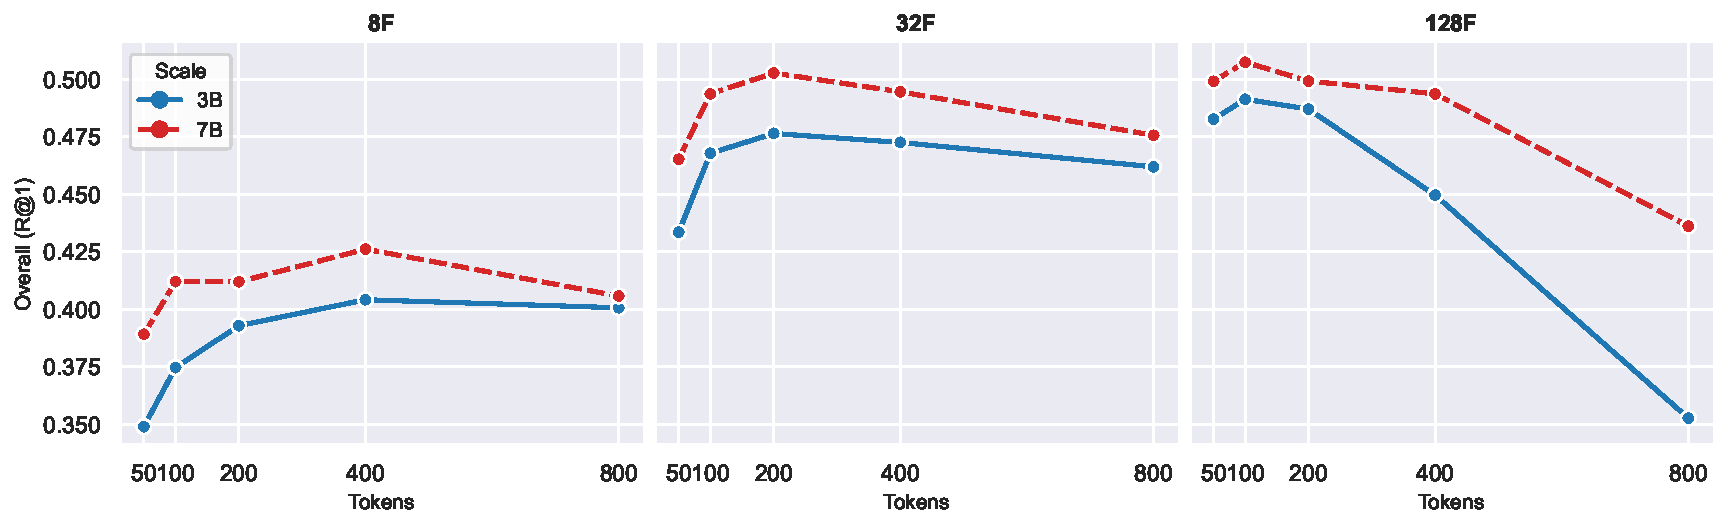
\includegraphics[width=\linewidth]{figures/mglvr/mglvr_testtime_spatial_scaling_1.pdf}
    \caption{Test-time spatial scaling sensitivity of GVE at temporal densities $F \in \{8, 32, 128\}$ frames per video. Each panel fixes $F$ and varies the number of spatial tokens $T$ per frame.}
    \label{mglvr:fig:spatial_scaling}
\end{figure}

\paragraph{Temporal Scaling.}
Varying $F$ from 4 to 512 frames reveals a divergence in scaling behavior across model families (Figure~\ref{mglvr:fig:temporal_scaling}). MLLM-based models exhibit continuous improvement up to $F = 128$, with the largest absolute gains on FN queries. CLIP-based models, by contrast, plateau around $F = 16$ and exhibit performance degradation on FN and MD queries at higher frame counts. This difference is consistent with the underlying architectural design: MLLM-based models process frames jointly through a transformer with positional encodings, whereas CLIP-based models aggregate frame-level features via mean pooling, which dilutes discriminative signals as $F$ increases.

\paragraph{Spatiotemporal Trade-off.}
When $N_{\text{total}}$ is held constant, the optimal allocation between $F$ and $T$ depends on query granularity (Figure~\ref{mglvr:fig:tradeoff}). CR queries favor high-resolution, low-frame-count configurations, while FN queries favor more frames at lower spatial resolution. Reducing spatial tokens primarily discards fine-grained texture while preserving semantic content, whereas reducing the number of frames risks eliminating visual evidence of brief events entirely.

\begin{sidewaysfigure}[t]
    \centering
    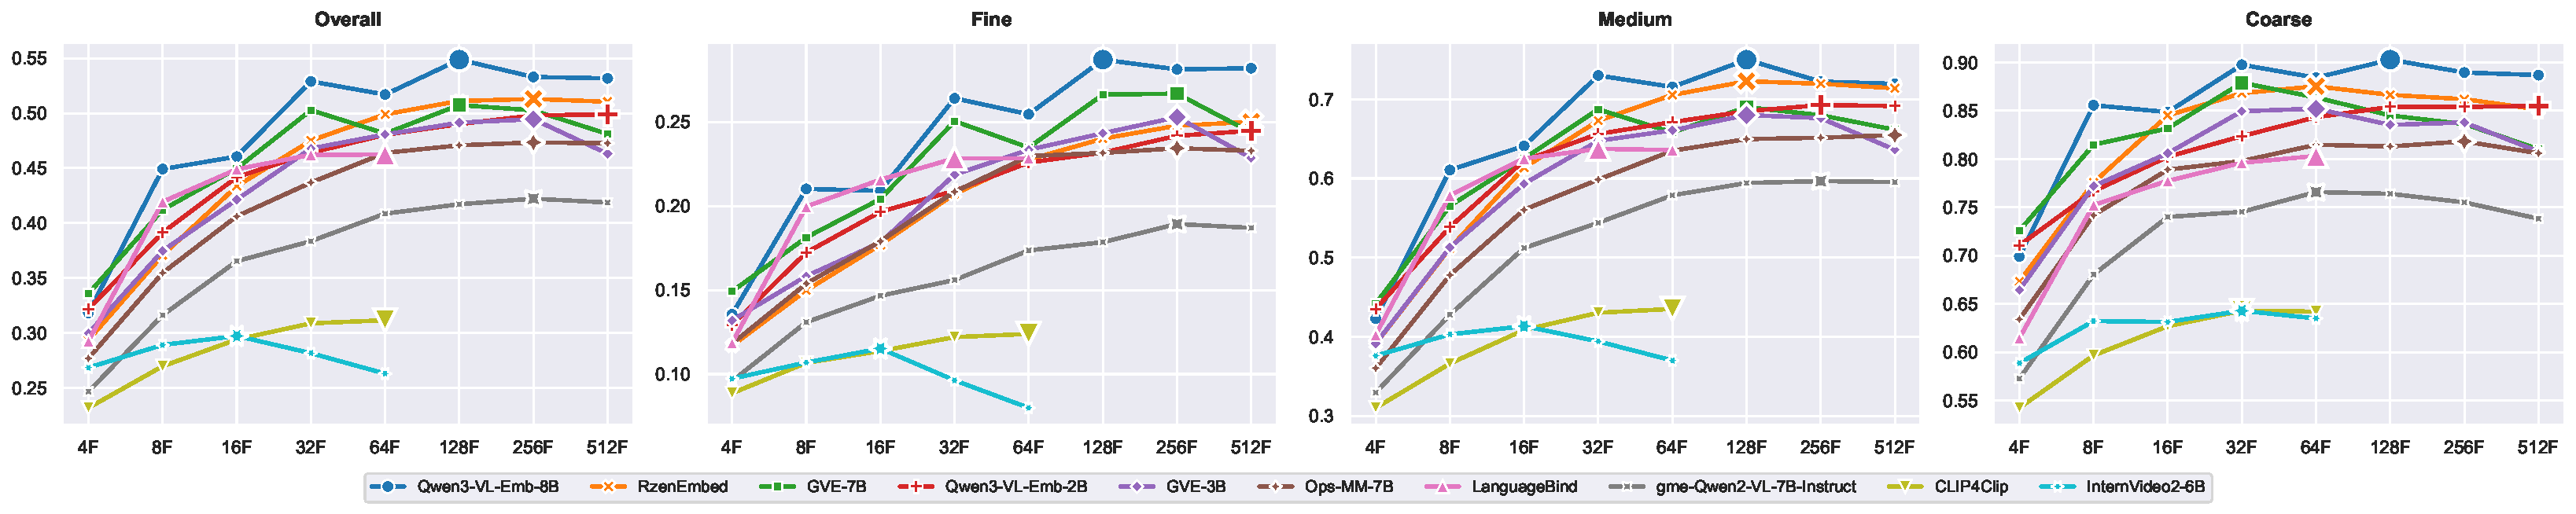
\includegraphics[width=\linewidth]{figures/mglvr/mglvr_testtime_temporal_scaling.pdf}
    \caption{Test-time temporal scaling across model families. MLLM-based models exhibit continuous improvement with increasing frame count, whereas CLIP-based models plateau and degrade at high frame counts.}
    \label{mglvr:fig:temporal_scaling}

    \vspace{1em}
    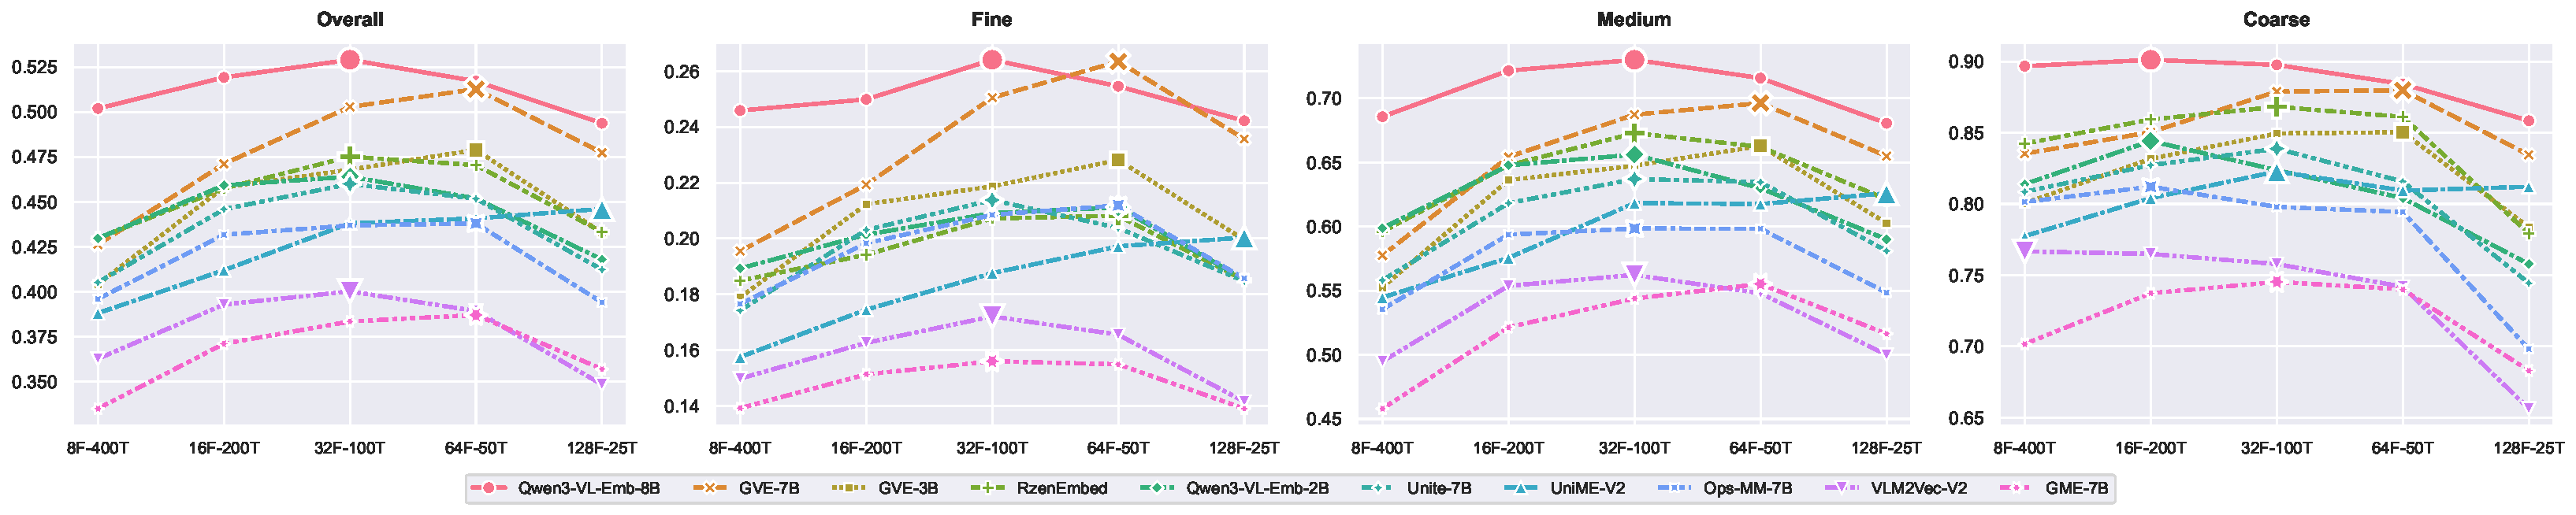
\includegraphics[width=\linewidth]{figures/mglvr/st_tradeoff.pdf}
    \caption{Retrieval performance under a fixed total token budget. The optimal allocation between spatial and temporal tokens shifts systematically with query granularity.}
    \label{mglvr:fig:tradeoff}
\end{sidewaysfigure}

\subsection{Training-Time Scaling}
\label{mglvr:sec:trainingtime}

Following the protocol of an existing work~\cite{guo2025gve}, we post-train Qwen2.5-VL-Instruct-3B~\cite{bai2025qwen25vl} with InfoNCE loss~\cite{oord2018representation} on 500K instances to examine how the training density $(F_{\text{train}}, T_{\text{train}})$ shapes the learned embedding space. We organize the results as two complementary comparisons. Table~\ref{mglvr:tab:train_spatial_scaling} varies the spatial training density and evaluates it at 4 and 8 test frames. Table~\ref{mglvr:tab:train_temporal_scaling} varies the temporal training density and evaluates it at 50 and 100 spatial tokens per test frame. Together, the two tables separate resolution robustness from frame-count anchoring.

\paragraph{Spatial Scaling: Resolution Robustness.}
Increasing $T_{\text{train}}$ yields consistent performance gains across most granularity levels and inference resolutions. Table~\ref{mglvr:tab:train_spatial_scaling}(a) reports evaluation at 4 test frames, and panel (b) verifies the same pattern at 8 test frames. Models trained at $T_{\text{train}} = 400$ achieve the best Overall R@1 in all four test-time spatial groups. Notably, even when evaluated at $T_{\text{test}} = 50$, the model trained at $T_{\text{train}} = 400$ substantially outperforms the model trained directly at $T_{\text{train}} = 50$ ($+0.0155$ Overall R@1). We term this property \textit{resolution robustness}: representations learned at high spatial density generalize effectively to low-density inference. However, this trend is not strictly monotonic at all granularity levels: at $T_{\text{test}} = 400$, increasing $T_{\text{train}}$ from 200 to 400 yields only marginal overall gains ($+0.0014$ Overall R@1) while slightly degrading Fine R@1 ($-0.0021$) and Coarse R@1 ($-0.0027$), suggesting diminishing returns at extreme spatial density.

\begin{table}[t]
    \centering
    \caption{Training-time spatial scaling with $F_{\text{train}}=4$, evaluated at (a) 4 and (b) 8 test frames. Models trained at $T_{\text{train}} \in \{50, 100, 200, 400\}$ are evaluated across all spatial test configurations. Bold indicates the best result within each group.}
    \label{mglvr:tab:train_spatial_scaling}
    \footnotesize
    \renewcommand{\arraystretch}{0.94}
    (a) Evaluation at 4 test frames.\par\smallskip
    \begin{tabular}{@{}c@{\hspace{3pt}}c@{\hspace{6pt}}c@{\hspace{3pt}}c@{\hspace{6pt}}*{7}{c@{\hspace{3pt}}}c@{}}
\toprule
\multicolumn{2}{c|}{Training} & \multicolumn{2}{c|}{Testing} & \multicolumn{2}{c|}{Overall} & \multicolumn{2}{c|}{FN} & \multicolumn{2}{c|}{MD} & \multicolumn{2}{c}{CR} \\
Temporal & Spatial & Temporal & Spatial & R@1   & MRR   & R@1   & MRR   & R@1   & MRR   & R@1   & MRR \\
\midrule
% --- Group 1: Test Spatial = 50T ---
\multirow{4}{*}{4F} & 50T & \multirow{4}{*}{4F} & \multirow{4}{*}{50T}  & 0.1941 & 0.2679 & 0.0731 & 0.1226 & 0.2591 & 0.3509 & 0.4613 & 0.5710 \\
& 100T & & & 0.2019 & 0.2770 & 0.0797 & 0.1298 & 0.2677 & 0.3617 & 0.4711 & 0.5811 \\
& 200T & & & 0.2060 & 0.2820 & 0.0837 & 0.1346 & 0.2714 & 0.3671 & 0.4773 & 0.5865 \\
& 400T & & & \textbf{0.2096} & \textbf{0.2851} & \textbf{0.0865} & \textbf{0.1378} & \textbf{0.2740} & \textbf{0.3687} & \textbf{0.4880} & \textbf{0.5939} \\
\midrule
% --- Group 2: Test Spatial = 100T ---
\multirow{4}{*}{4F} & 50T & \multirow{4}{*}{4F} & \multirow{4}{*}{100T} & 0.2243 & 0.3011 & 0.0865 & 0.1390 & 0.2996 & 0.3968 & 0.5236 & 0.6277 \\
& 100T & & & 0.2212 & 0.2979 & 0.0837 & 0.1375 & 0.2945 & 0.3901 & 0.5272 & 0.6299 \\
& 200T & & & 0.2384 & 0.3180 & 0.0922 & 0.1494 & 0.3182 & 0.4173 & 0.5565 & 0.6583 \\
& 400T & & & \textbf{0.2474} & \textbf{0.3262} & \textbf{0.0975} & \textbf{0.1558} & \textbf{0.3300} & \textbf{0.4267} & \textbf{0.5708} & \textbf{0.6696} \\
\midrule
% --- Group 3: Test Spatial = 200T ---
\multirow{4}{*}{4F} & 50T & \multirow{4}{*}{4F} & \multirow{4}{*}{200T} & 0.2406 & 0.3168 & 0.0890 & 0.1420 & 0.3199 & 0.4178 & 0.5833 & 0.6764 \\
& 100T & & & 0.2425 & 0.3202 & 0.0922 & 0.1473 & 0.3197 & 0.4187 & 0.5877 & 0.6820 \\
& 200T & & & 0.2454 & 0.3230 & 0.0948 & 0.1500 & 0.3238 & 0.4220 & 0.5877 & 0.6834 \\
& 400T & & & \textbf{0.2581} & \textbf{0.3385} & \textbf{0.1031} & \textbf{0.1628} & \textbf{0.3440} & \textbf{0.4425} & \textbf{0.5913} & \textbf{0.6910} \\
\midrule
% --- Group 4: Test Spatial = 400T ---
\multirow{4}{*}{4F} & 50T & \multirow{4}{*}{4F} & \multirow{4}{*}{400T} & 0.2503 & 0.3263 & 0.0926 & 0.1471 & 0.3353 & 0.4318 & \textbf{0.5975} & 0.6883 \\
& 100T & & & 0.2507 & 0.3285 & 0.0914 & 0.1501 & 0.3378 & 0.4332 & \textbf{0.5975} & 0.6898 \\
& 200T & & & 0.2561 & 0.3342 & \textbf{0.0984} & \textbf{0.1566} & 0.3431 & 0.4392 & 0.5966 & \textbf{0.6909} \\
& 400T & & & \textbf{0.2575} & \textbf{0.3359} & 0.0963 & 0.1563 & \textbf{0.3496} & \textbf{0.4442} & 0.5939 & 0.6889 \\
\bottomrule
\end{tabular}
\par\medskip
(b) Evaluation at 8 test frames.\par\smallskip
\begin{tabular}{@{}c@{\hspace{3pt}}c@{\hspace{6pt}}c@{\hspace{3pt}}c@{\hspace{6pt}}*{7}{c@{\hspace{3pt}}}c@{}}
\toprule
\multicolumn{2}{c|}{Training} & \multicolumn{2}{c|}{Testing} & \multicolumn{2}{c|}{Overall} & \multicolumn{2}{c|}{FN} & \multicolumn{2}{c|}{MD} & \multicolumn{2}{c}{CR} \\
Temporal & Spatial & Temporal & Spatial & R@1 & MRR & R@1 & MRR & R@1 & MRR & R@1 & MRR \\
\midrule
\multirow{4}{*}{4F} & 50T  & \multirow{4}{*}{8F} & \multirow{4}{*}{50T}  & 0.2523 & 0.3349 & 0.0941 & 0.1561 & 0.3438 & 0.4461 & 0.5779 & 0.6746 \\
                    & 100T &                      &                       & 0.2567 & 0.3392 & 0.1018 & 0.1620 & 0.3486 & 0.4512 & 0.5672 & 0.6685 \\
                    & 200T &                      &                       & 0.2702 & 0.3529 & 0.1130 & 0.1734 & 0.3607 & 0.4647 & 0.5948 & 0.6928 \\
                    & 400T &                      &                       & \textbf{0.2778} & \textbf{0.3610} & \textbf{0.1137} & \textbf{0.1780} & \textbf{0.3759} & \textbf{0.4773} & \textbf{0.6037} & \textbf{0.6991} \\
\midrule
\multirow{4}{*}{4F} & 50T  & \multirow{4}{*}{8F} & \multirow{4}{*}{100T} & 0.2773 & 0.3598 & 0.1028 & 0.1673 & 0.3793 & 0.4817 & 0.6322 & 0.7169 \\
                    & 100T &                      &                       & 0.2815 & 0.3612 & 0.1065 & 0.1683 & 0.3877 & 0.4851 & 0.6233 & 0.7122 \\
                    & 200T &                      &                       & 0.2907 & 0.3709 & 0.1107 & 0.1752 & 0.3993 & 0.4962 & 0.6447 & 0.7292 \\
                    & 400T &                      &                       & \textbf{0.3041} & \textbf{0.3871} & \textbf{0.1220} & \textbf{0.1897} & \textbf{0.4179} & \textbf{0.5169} & \textbf{0.6474} & \textbf{0.7357} \\
\midrule
\multirow{4}{*}{4F} & 50T  & \multirow{4}{*}{8F} & \multirow{4}{*}{200T} & 0.2889 & 0.3704 & 0.1037 & 0.1691 & 0.4015 & 0.5008 & 0.6500 & 0.7333 \\
                    & 100T &                      &                       & 0.2915 & 0.3721 & 0.1109 & 0.1740 & 0.4000 & 0.4991 & 0.6483 & 0.7341 \\
                    & 200T &                      &                       & 0.2970 & 0.3785 & 0.1105 & 0.1767 & 0.4085 & 0.5076 & 0.6670 & 0.7480 \\
                    & 400T &                      &                       & \textbf{0.3062} & \textbf{0.3883} & \textbf{0.1171} & \textbf{0.1851} & \textbf{0.4242} & \textbf{0.5224} & \textbf{0.6634} & \textbf{0.7453} \\
\midrule
\multirow{4}{*}{4F} & 50T  & \multirow{4}{*}{8F} & \multirow{4}{*}{400T} & 0.2936 & 0.3738 & 0.1041 & 0.1681 & 0.4090 & 0.5076 & 0.6616 & 0.7423 \\
                    & 100T &                      &                       & 0.2977 & 0.3778 & 0.1124 & 0.1754 & 0.4097 & 0.5086 & 0.6607 & 0.7435 \\
                    & 200T &                      &                       & 0.3001 & 0.3800 & 0.1171 & 0.1790 & 0.4090 & 0.5085 & 0.6652 & 0.7488 \\
                    & 400T &                      &                       & \textbf{0.3058} & \textbf{0.3861} & \textbf{0.1203} & \textbf{0.1843} & \textbf{0.4198} & \textbf{0.5175} & \textbf{0.6625} & \textbf{0.7469} \\
\bottomrule
\end{tabular}
\end{table}

\FloatBarrier
\paragraph{Temporal Scaling: Frame-Count Anchoring.}
Unlike spatial representations, temporal representations are tightly coupled to the frame count seen during training, a phenomenon we term \textit{frame-count anchoring}. Table~\ref{mglvr:tab:train_temporal_scaling} shows that the pattern persists when evaluated at 50 and 100 spatial tokens per frame in panels (a) and (b), respectively. A mismatch between $F_{\text{train}}$ and $F_{\text{test}}$ consistently degrades performance in both directions, but the degradation is asymmetric. When $F_{\text{train}} \gg F_{\text{test}}$, the performance drop is more severe: a model trained at $F_{\text{train}} = 32$ and evaluated at $F_{\text{test}} = 4$ drops $0.0104$ in Fine R@1 relative to the matched $F_{\text{train}} = 4$ baseline (Group~1 in Table~\ref{mglvr:tab:train_temporal_scaling}(a)). In the inverse direction, a model trained at $F_{\text{train}} = 4$ and evaluated at $F_{\text{test}} = 32$ drops $0.0083$ in Fine R@1 relative to the matched $F_{\text{train}} = 32$ baseline (Group~4 in Table~\ref{mglvr:tab:train_temporal_scaling}(a)). Although these gaps are measured against different absolute performance levels and should be interpreted accordingly, the consistent pattern across groups suggests that low-frame-count training better preserves fine-grained discriminability under temporal mismatch than high-frame-count training does.

\begin{table}[t]
    \centering
    \caption{Training-time temporal scaling with $T_{\text{train}}=50$, evaluated at (a) 50 and (b) 100 spatial tokens per test frame. Models trained at $F_{\text{train}} \in \{4, 8, 16, 32\}$ are evaluated across six temporal test configurations. Bold indicates the best result within each group.}
    \label{mglvr:tab:train_temporal_scaling}
    \footnotesize
    \renewcommand{\arraystretch}{0.78}
    (a) Evaluation at 50 spatial tokens per test frame.\par\smallskip
    \begin{tabular}{@{}c@{\hspace{3pt}}c@{\hspace{6pt}}c@{\hspace{3pt}}c@{\hspace{6pt}}*{7}{c@{\hspace{3pt}}}c@{}}
\toprule
\multicolumn{2}{c|}{Training} & \multicolumn{2}{c|}{Testing} & \multicolumn{2}{c|}{Overall} & \multicolumn{2}{c|}{FN} & \multicolumn{2}{c|}{MD} & \multicolumn{2}{c}{CR} \\
Temporal & Spatial & Temporal & Spatial & R@1   & MRR   & R@1   & MRR   & R@1   & MRR   & R@1   & MRR \\
\midrule
% --- Group 1: Test Temporal = 4F ---
4F  & \multirow{4}{*}{50T} & \multirow{4}{*}{4F} & \multirow{4}{*}{50T} & 0.2076 & 0.2837 & 0.0841 & 0.1352 & \textbf{0.2706} & \textbf{0.3666} & 0.4924 & 0.6002 \\
8F  & & & & 0.2080 & 0.2842 & 0.0858 & 0.1374 & 0.2694 & 0.3654 & \textbf{0.4933} & \textbf{0.6004} \\
16F & & & & \textbf{0.2082} & \textbf{0.2854} & \textbf{0.0882} & \textbf{0.1396} & 0.2677 & 0.3659 & 0.4915 & 0.5987 \\
32F & & & & 0.1930 & 0.2687 & 0.0737 & 0.1261 & 0.2528 & 0.3466 & 0.4720 & 0.5792 \\
\midrule
% --- Group 2: Test Temporal = 8F ---
4F  & \multirow{4}{*}{50T} & \multirow{4}{*}{8F} & \multirow{4}{*}{50T} & 0.2639 & 0.3515 & 0.1054 & 0.1694 & 0.3566 & 0.4669 & 0.5859 & 0.6892 \\
8F  & & & & \textbf{0.2741} & \textbf{0.3605} & \textbf{0.1143} & \textbf{0.1788} & \textbf{0.3667} & \textbf{0.4764} & \textbf{0.6020} & \textbf{0.6946} \\
16F & & & & 0.2486 & 0.3295 & 0.0992 & 0.1591 & 0.3281 & 0.4291 & 0.5815 & 0.6763 \\
32F & & & & 0.2390 & 0.3168 & 0.0982 & 0.1531 & 0.3117 & 0.4095 & 0.5610 & 0.6614 \\
\midrule
% --- Group 3: Test Temporal = 16F ---
4F  & \multirow{4}{*}{50T} & \multirow{4}{*}{16F} & \multirow{4}{*}{50T} & 0.3165 & 0.4086 & 0.1207 & 0.1951 & 0.4464 & 0.5590 & 0.6581 & 0.7484 \\
8F  & & & & 0.3071 & 0.3941 & 0.1147 & 0.1839 & 0.4288 & 0.5363 & 0.6643 & 0.7501 \\
16F & & & & \textbf{0.3254} & \textbf{0.4136} & \textbf{0.1235} & \textbf{0.1972} & \textbf{0.4587} & \textbf{0.5648} & \textbf{0.6803} & \textbf{0.7628} \\
32F & & & & 0.3090 & 0.3987 & 0.1196 & 0.1903 & 0.4254 & 0.5385 & 0.6732 & 0.7560 \\
\midrule
% --- Group 4: Test Temporal = 32F ---
4F  & \multirow{4}{*}{50T} & \multirow{4}{*}{32F} & \multirow{4}{*}{50T} & 0.3310 & 0.4196 & 0.1373 & 0.2088 & 0.4611 & 0.5678 & 0.6625 & 0.7559 \\
8F  & & & & 0.3556 & 0.4433 & 0.1432 & 0.2192 & 0.5017 & 0.6057 & 0.7070 & 0.7831 \\
16F & & & & 0.3574 & 0.4466 & \textbf{0.1466} & \textbf{0.2255} & 0.5034 & 0.6068 & 0.7026 & 0.7820 \\
32F & & & & \textbf{0.3596} & \textbf{0.4476} & 0.1456 & 0.2224 & \textbf{0.5075} & \textbf{0.6118} & \textbf{0.7115} & \textbf{0.7857} \\
\midrule
% --- Group 5: Test Temporal = 64F ---
4F  & \multirow{4}{*}{50T} & \multirow{4}{*}{64F} & \multirow{4}{*}{50T} & 0.3829 & 0.4717 & 0.1655 & 0.2440 & 0.5328 & 0.6392 & \textbf{0.7409} & \textbf{0.8110} \\
8F  & & & & 0.3772 & 0.4640 & 0.1596 & 0.2375 & 0.5280 & 0.6294 & 0.7329 & 0.8031 \\
16F & & & & 0.3877 & 0.4746 & \textbf{0.1698} & \textbf{0.2488} & 0.5420 & 0.6421 & 0.7320 & 0.8026 \\
32F & & & & \textbf{0.3892} & \textbf{0.4769} & 0.1668 & 0.2472 & \textbf{0.5468} & \textbf{0.6472} & 0.7400 & \textbf{0.8110} \\
\midrule
% --- Group 6: Test Temporal = 128F ---
4F  & \multirow{4}{*}{50T} & \multirow{4}{*}{128F} & \multirow{4}{*}{50T} & 0.4021 & 0.4900 & 0.1772 & 0.2604 & 0.5633 & 0.6626 & 0.7498 & 0.8174 \\
8F  & & & & 0.3941 & 0.4799 & 0.1698 & 0.2511 & 0.5538 & 0.6500 & 0.7453 & 0.8116 \\
16F & & & & 0.4058 & 0.4939 & 0.1806 & 0.2651 & \textbf{0.5681} & \textbf{0.6661} & 0.7507 & 0.8174 \\
32F & & & & \textbf{0.4078} & \textbf{0.4949} & \textbf{0.1859} & \textbf{0.2695} & 0.5666 & 0.6629 & \textbf{0.7516} & \textbf{0.8195} \\
\bottomrule
\end{tabular}
\par\medskip
(b) Evaluation at 100 spatial tokens per test frame.\par\smallskip
\begin{tabular}{@{}c@{\hspace{3pt}}c@{\hspace{6pt}}c@{\hspace{3pt}}c@{\hspace{6pt}}*{7}{c@{\hspace{3pt}}}c@{}}
\toprule
\multicolumn{2}{c|}{Training} & \multicolumn{2}{c|}{Testing} & \multicolumn{2}{c|}{Overall} & \multicolumn{2}{c|}{FN} & \multicolumn{2}{c|}{MD} & \multicolumn{2}{c}{CR} \\
Temporal & Spatial & Temporal & Spatial & R@1 & MRR & R@1 & MRR & R@1 & MRR & R@1 & MRR \\
\midrule
4F  & \multirow{4}{*}{50T} & \multirow{4}{*}{4F}   & \multirow{4}{*}{100T} & \textbf{0.2426} & \textbf{0.3213} & \textbf{0.0935} & \textbf{0.1498} & \textbf{0.3230} & \textbf{0.4222} & \textbf{0.5708} & \textbf{0.6681} \\
8F  &                      &                       &                       & 0.2395 & 0.3189 & 0.0912 & 0.1490 & 0.3213 & 0.4193 & 0.5592 & 0.6609 \\
16F &                      &                       &                       & 0.2251 & 0.3008 & 0.0861 & 0.1408 & 0.2945 & 0.3891 & 0.5512 & 0.6456 \\
32F &                      &                       &                       & 0.2286 & 0.3031 & 0.0916 & 0.1440 & 0.2970 & 0.3908 & 0.5503 & 0.6459 \\
\midrule
4F  & \multirow{4}{*}{50T} & \multirow{4}{*}{8F}   & \multirow{4}{*}{100T} & 0.3116 & 0.3984 & 0.1232 & 0.1943 & 0.4336 & 0.5367 & 0.6509 & 0.7438 \\
8F  &                      &                       &                       & \textbf{0.3188} & \textbf{0.4027} & \textbf{0.1288} & \textbf{0.1979} & \textbf{0.4384} & \textbf{0.5390} & \textbf{0.6741} & \textbf{0.7582} \\
16F &                      &                       &                       & 0.2982 & 0.3828 & 0.1169 & 0.1846 & 0.4116 & 0.5126 & 0.6394 & 0.7345 \\
32F &                      &                       &                       & 0.3045 & 0.3892 & 0.1258 & 0.1925 & 0.4112 & 0.5151 & 0.6598 & 0.7493 \\
\midrule
4F  & \multirow{4}{*}{50T} & \multirow{4}{*}{16F}  & \multirow{4}{*}{100T} & 0.3549 & 0.4422 & 0.1392 & 0.2160 & 0.4988 & 0.6026 & \textbf{0.7284} & \textbf{0.7986} \\
8F  &                      &                       &                       & 0.3553 & 0.4426 & 0.1400 & 0.2172 & 0.5010 & 0.6035 & 0.7204 & 0.7942 \\
16F &                      &                       &                       & \textbf{0.3582} & \textbf{0.4454} & \textbf{0.1405} & \textbf{0.2176} & \textbf{0.5097} & \textbf{0.6114} & 0.7124 & 0.7882 \\
32F &                      &                       &                       & 0.3266 & 0.4116 & 0.1194 & 0.1896 & 0.4611 & 0.5642 & 0.6990 & 0.7793 \\
\midrule
4F  & \multirow{4}{*}{50T} & \multirow{4}{*}{32F}  & \multirow{4}{*}{100T} & 0.3860 & 0.4736 & 0.1619 & 0.2404 & 0.5432 & 0.6462 & 0.7453 & 0.8138 \\
8F  &                      &                       &                       & 0.3805 & 0.4663 & 0.1594 & 0.2362 & 0.5340 & 0.6345 & 0.7409 & 0.8104 \\
16F &                      &                       &                       & \textbf{0.3905} & \textbf{0.4783} & \textbf{0.1664} & \textbf{0.2465} & 0.5483 & \textbf{0.6496} & \textbf{0.7480} & \textbf{0.8179} \\
32F &                      &                       &                       & 0.3877 & 0.4741 & 0.1636 & 0.2434 & \textbf{0.5495} & 0.6457 & 0.7302 & 0.8078 \\
\midrule
4F  & \multirow{4}{*}{50T} & \multirow{4}{*}{64F}  & \multirow{4}{*}{100T} & 0.4086 & 0.4923 & 0.1728 & 0.2538 & \textbf{0.5799} & \textbf{0.6726} & 0.7649 & 0.8266 \\
8F  &                      &                       &                       & 0.3960 & 0.4809 & 0.1696 & 0.2485 & 0.5560 & 0.6530 & 0.7551 & 0.8199 \\
16F &                      &                       &                       & 0.4108 & 0.4961 & 0.1832 & 0.2627 & 0.5739 & 0.6713 & 0.7631 & 0.8284 \\
32F &                      &                       &                       & \textbf{0.4148} & \textbf{0.4994} & \textbf{0.1885} & \textbf{0.2693} & 0.5739 & 0.6699 & \textbf{0.7765} & \textbf{0.8347} \\
\midrule
4F  & \multirow{4}{*}{50T} & \multirow{4}{*}{128F} & \multirow{4}{*}{100T} & 0.4130 & 0.4970 & 0.1859 & 0.2660 & 0.5794 & 0.6723 & 0.7507 & 0.8186 \\
8F  &                      &                       &                       & 0.4013 & 0.4853 & 0.1764 & 0.2556 & 0.5618 & 0.6569 & 0.7516 & 0.8143 \\
16F &                      &                       &                       & 0.4167 & 0.5015 & 0.1840 & 0.2679 & \textbf{0.5843} & 0.6769 & 0.7738 & 0.8330 \\
32F &                      &                       &                       & \textbf{0.4226} & \textbf{0.5073} & \textbf{0.1951} & \textbf{0.2782} & \textbf{0.5843} & \textbf{0.6782} & \textbf{0.7801} & \textbf{0.8368} \\
\bottomrule
\end{tabular}
\end{table}

\FloatBarrier
\subsection{Error Analysis and Case Studies}
\label{mglvr:sec:error_analysis}

The aggregate scaling results reveal how performance changes with sampling density, but they do not show how individual failures arise. Figure~\ref{mglvr:fig:error_cases} summarizes three representative retrieval cases that delimit both the benefits and the limitations of spatiotemporal scaling.

\paragraph{Degradation on Long Continuous Temporal Segments.}
As shown in Figure~\ref{mglvr:fig:error1}, performance degrades on long, continuous events. A fixed-length context window, such as 16 frames, divides a long video into short and independently processed clips, which can prevent the representation from capturing the full temporal scope of events spanning multiple clips.

\paragraph{Failure in Fine-Grained Temporal Retrieval.}
Figure~\ref{mglvr:fig:error2} shows a case in which the target event is a brief scene in the background. This resembles a needle-in-a-haystack setting, where increasing temporal coverage can improve the chance of observing the event but does not guarantee that the representation will preserve it strongly enough for retrieval.

\paragraph{Incomplete Satisfaction of Semantic Constraints.}
As shown in Figure~\ref{mglvr:fig:error3}, the model sometimes fails to satisfy all query conditions. The top-1 retrieved video satisfies the ``speaker'' requirement but does not match the ``blue background'' constraint. Similarly, the top-3 retrieved video satisfies most constraints but misses the requirement that the speaker wear a patterned shirt.

\begin{figure}[t]
  \centering
  \subfloat[]{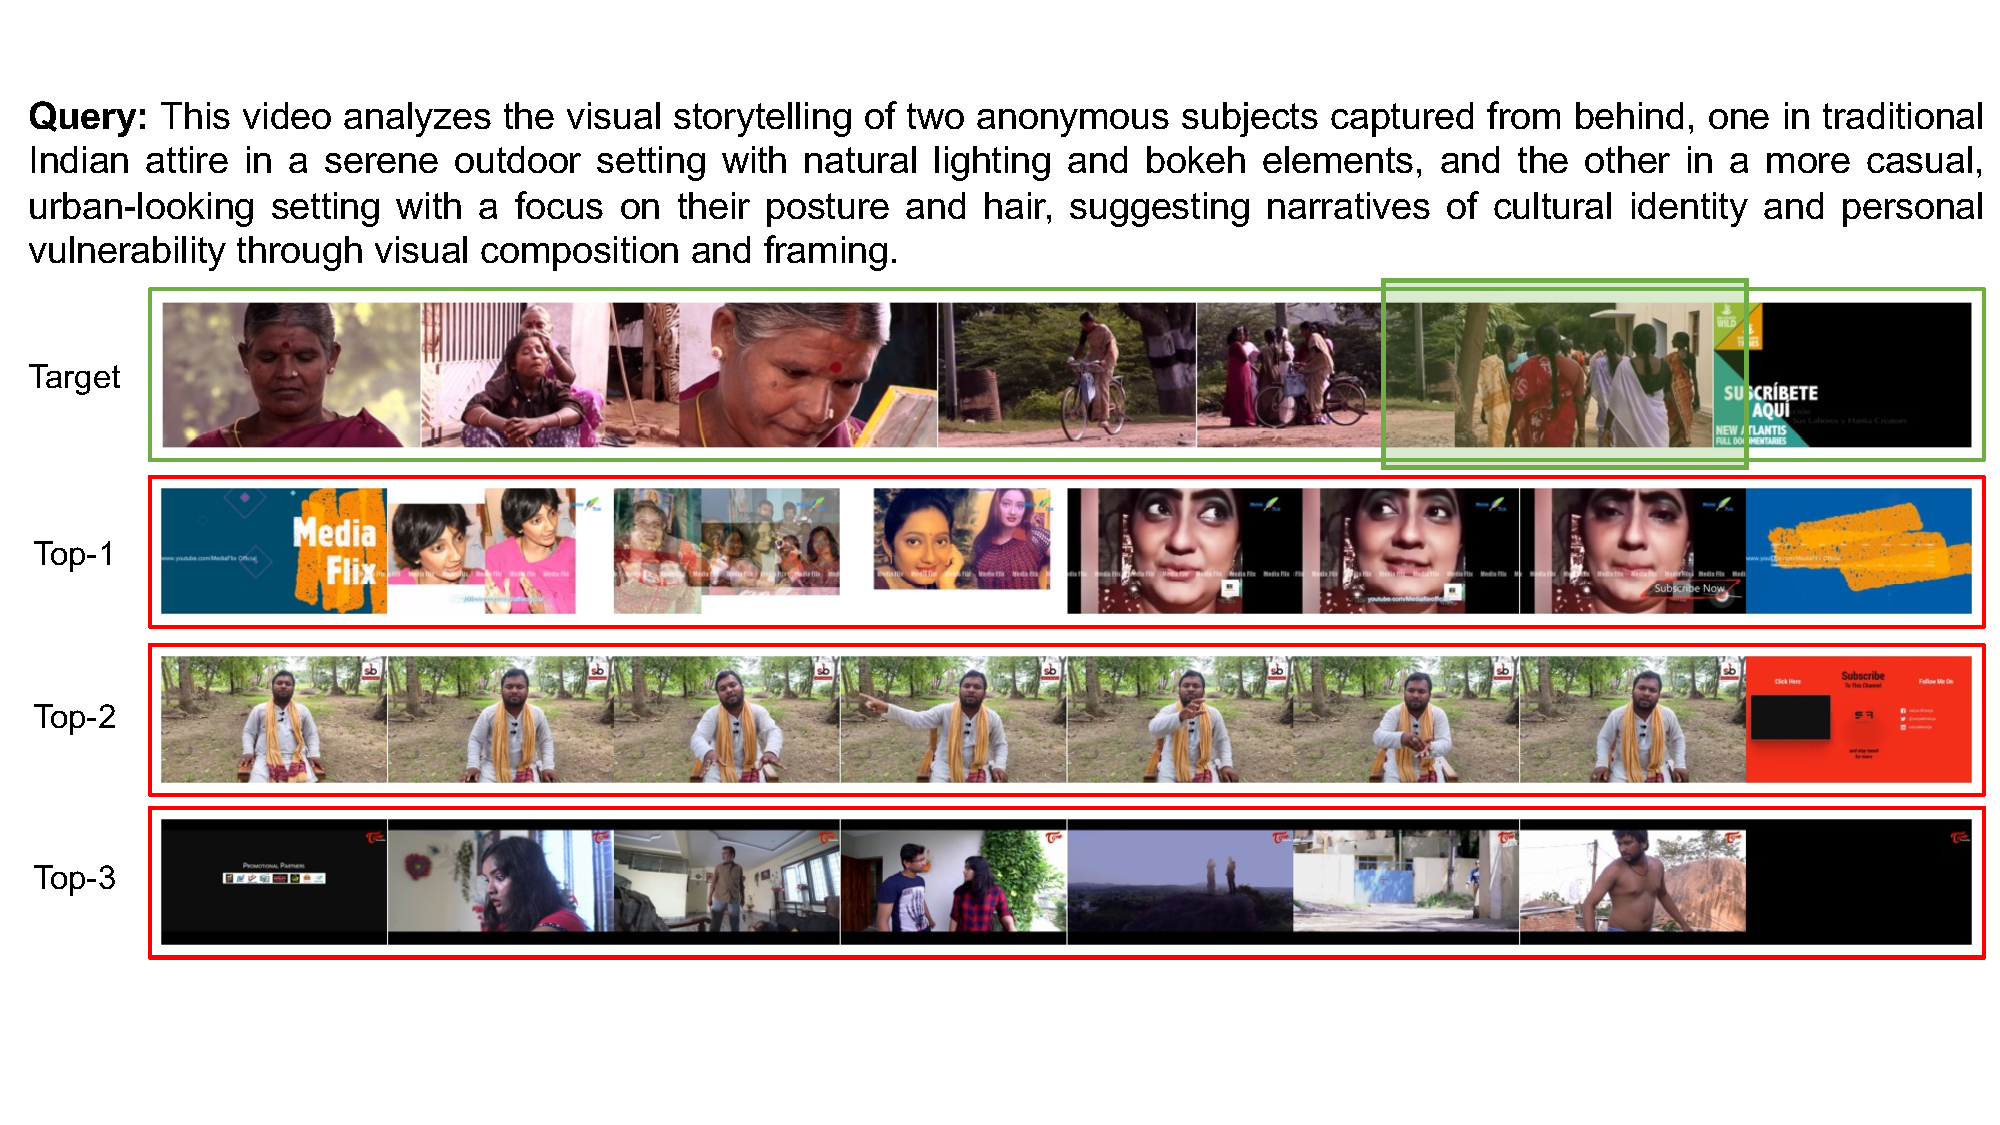
\includegraphics[width=\linewidth]{figures/mglvr/error-analysis/lvr-error-analysis-1.pdf}\label{mglvr:fig:error1}}\\[-0.5ex]
  \subfloat[]{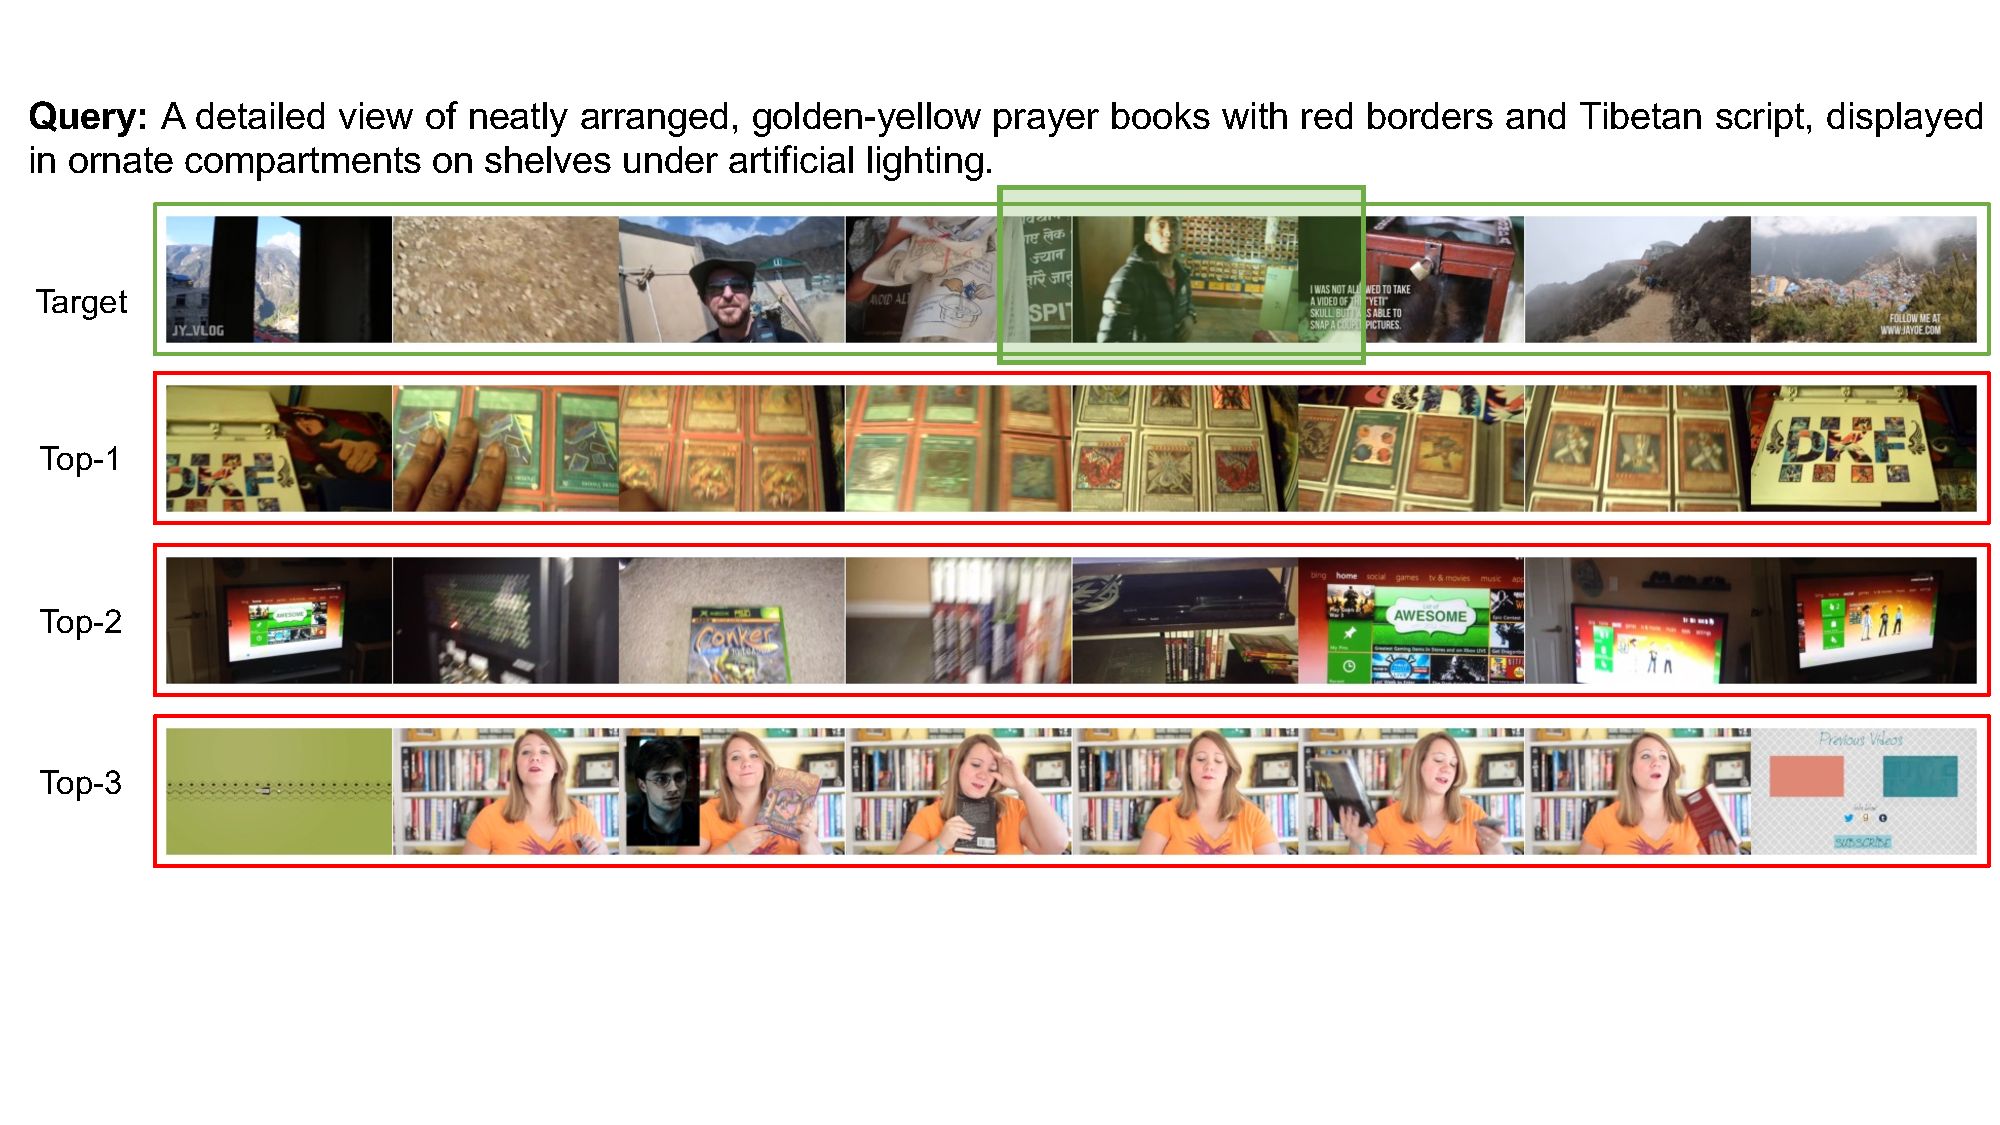
\includegraphics[width=\linewidth]{figures/mglvr/error-analysis/lvr-error-analysis-2.pdf}\label{mglvr:fig:error2}}\\[-0.5ex]
  \subfloat[]{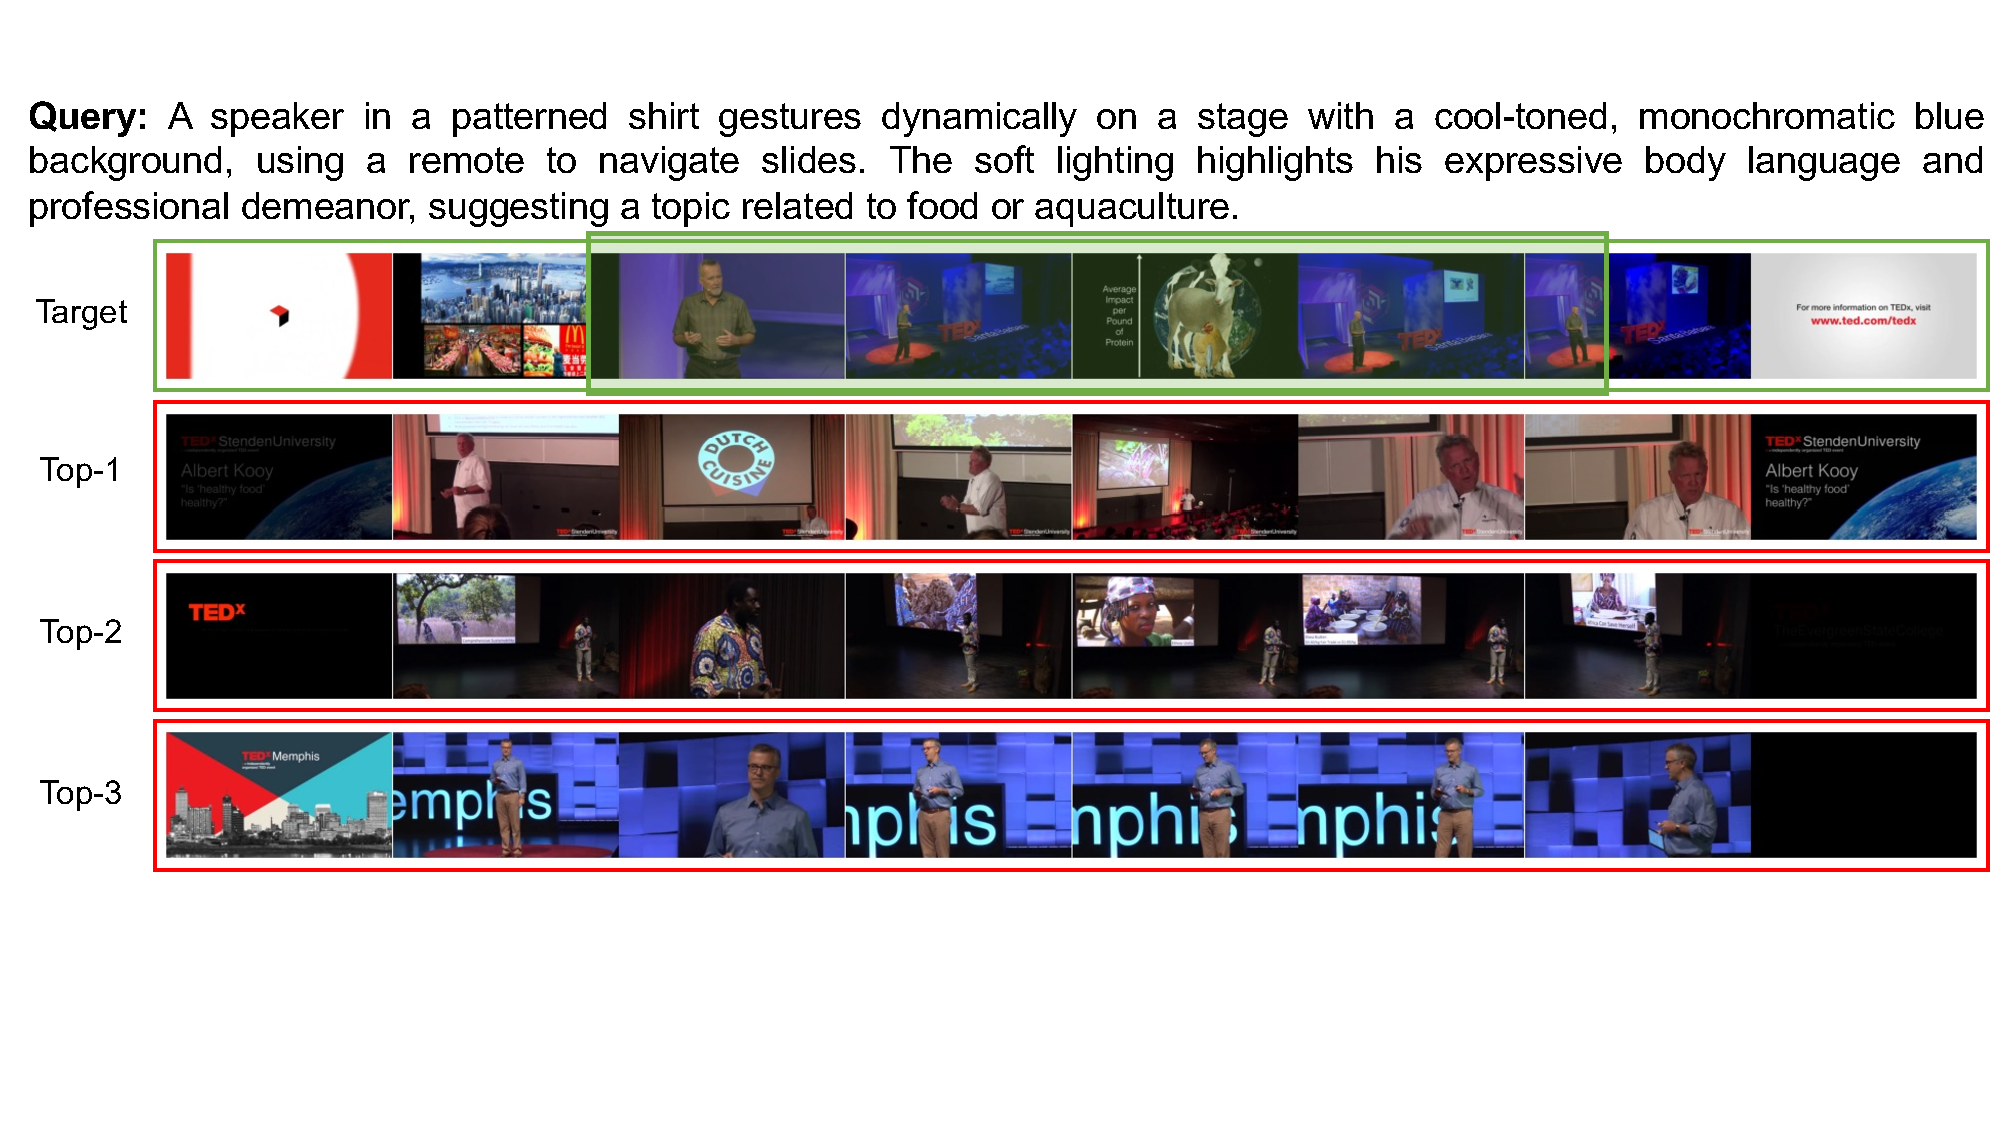
\includegraphics[width=\linewidth]{figures/mglvr/error-analysis/lvr-error-analysis-3.pdf}\label{mglvr:fig:error3}}
  \caption{Representative retrieval errors: (a) degradation on long continuous temporal segments, (b) failure in fine-grained temporal retrieval, and (c) incomplete satisfaction of semantic constraints.}
  \label{mglvr:fig:error_cases}
\end{figure}

\FloatBarrier
\section[VEterfall: Channeling Scaling Potential for Self-Enhancement of Video Embedding Models]{VEterfall: Channeling Scaling Potential for\\Self-Enhancement of Video Embedding Models}
\label{mglvr:sec:veterfall}

Our analysis reveals a key asymmetry: spatial embeddings tolerate token compression well, whereas temporal ones are governed by frame-count anchoring, i.e., models evaluated with high frame-density inputs degrade when the frame count is reduced at inference time. This suggests that the knowledge required for low-density inference is already latent within representations produced under high-density input sampling, but is not automatically transferred when the sampling configuration changes. We therefore propose \textbf{Video Embedding Waterfall (VEterfall)}, a progressive dense-to-sparse self-distillation framework that explicitly propagates this knowledge along the sampling-density axis, from high- to low-density configurations stage by stage, analogous to water descending through successive levels of a waterfall as shown in Figure~\ref{mglvr:fig:veterfall}.

\subsection{Method}

\paragraph{Single Dense-to-Sparse Distillation Step.}
The basic unit of VEterfall is a single distillation step~\cite{hinton2015distilling} from a denser to a sparser input sampling configuration, where density refers jointly to the number of frames sampled from the video and the number of spatial tokens retained per frame at inference time. A frozen teacher processes inputs at higher sampling density, while a student with the same architecture and initialization from the same pre-trained checkpoint $\mathcal{V}^{(0)}$ (here GVE-3B~\cite{guo2025gve}) is trained at a strictly lower density. The student is optimized to align its video embedding with that of the teacher via MSE loss, with an additional InfoNCE~\cite{oord2018representation} loss term ($\lambda{=}0.5$) to maintain video-text alignment by contrastive learning throughout density reduction.

\begin{figure}[t]
    \centering
    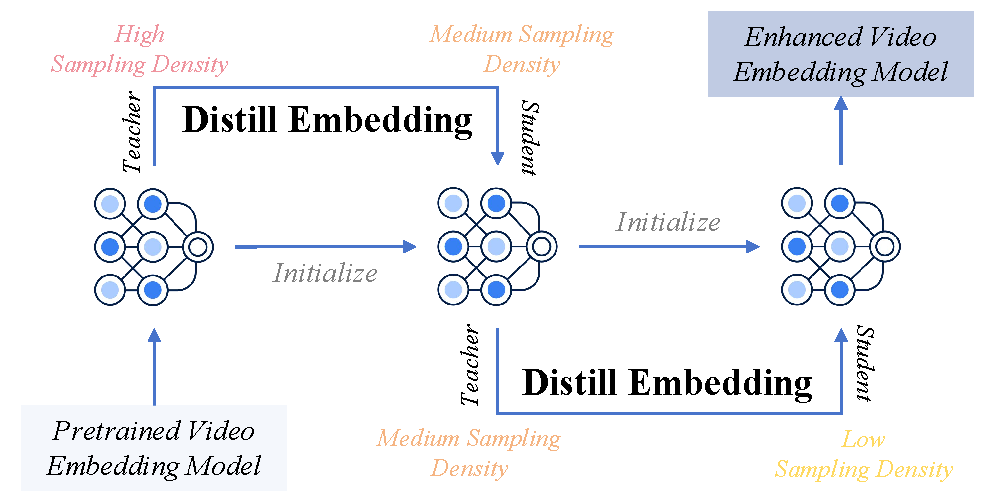
\includegraphics[width=0.75\linewidth]{figures/mglvr/d2s.pdf}
    \caption{VEterfall progressively distills video embeddings across progressively sparser input sampling configurations using the pretrained model itself as the teacher at each stage.}
    \label{mglvr:fig:veterfall}
\end{figure}

\paragraph{$K$-Round Cascade.}
To support large overall density reductions while keeping each individual step within a reliable transfer range, VEterfall chains $K$ distillation steps into a cascade, where each round takes the previous checkpoint as its frozen teacher:
\begin{equation*}
\mathcal{V}^{(k)} \xleftarrow{\;\text{distill}\;} \mathcal{V}^{(k-1)},
\qquad k = 1, \dots, K.
\end{equation*}
Here $\mathcal{V}^{(0)}$ serves as the pre-trained video embedding model, and $K$ controls the granularity of the reduction schedule.

\paragraph{Instantiation.}
We set $K{=}2$. Starting from $\mathcal{V}^{(0)}$ at $(16\text{F},\,400\text{T})$, the first round produces $\mathcal{V}^{(1)}$ at $(8\text{F},\,200\text{T})$, and the second produces $\mathcal{V}^{(2)}$ at $(4\text{F},\,100\text{T})$. Across two rounds, the input token budget is reduced by $16\times$ with no modification to the inference architecture. Each round uses 100K text-video pairs from InternVid~\cite{wang2023internvid}, a substantially smaller data requirement than comparable models.

\subsection{Experiments}

\begin{table}[t]
    \centering
    \caption{\textbf{Iterative Distillation.} R@1 performance across successive rounds ($K=1, 2$). VEterfall effectively recovers performance at lower densities, particularly for fine-grained queries.}
    \label{mglvr:tab:distillation}
    \begin{tabular}{@{}ll|*{4}{c}@{}}
        \toprule
        Setting & Model & Overall & Fine & Medium & Coarse \\
        \midrule
        \multirow{3}{*}{16F-400T} 
          & $\mathcal{V}^{(0)}$ & 0.447 & 0.202 & 0.622 & \textbf{0.829} \\
          & $\mathcal{V}^{(1)}$ & \underline{0.454} & \underline{0.212} & \underline{0.628} & \underline{0.826} \\
          & $\mathcal{V}^{(2)}$ & \textbf{0.456} & \textbf{0.215} & \textbf{0.630} & 0.819 \\
        \cmidrule(lr){1-6}
        \multirow{3}{*}{8F-200T} 
          & $\mathcal{V}^{(0)}$ & 0.369 & 0.148 & 0.508 & \textbf{0.782} \\
          & $\mathcal{V}^{(1)}$ & \underline{0.398} & \underline{0.182} & \underline{0.540} & \underline{0.780} \\
          & $\mathcal{V}^{(2)}$ & \textbf{0.402} & \textbf{0.188} & \textbf{0.543} & 0.777 \\
        \cmidrule(lr){1-6}
        \multirow{3}{*}{4F-100T} 
          & $\mathcal{V}^{(0)}$ & 0.300 & \underline{0.132} & 0.391 & \underline{0.664} \\
          & $\mathcal{V}^{(1)}$ & \underline{0.300} & 0.130 & \underline{0.394} & \underline{0.664} \\
          & $\mathcal{V}^{(2)}$ & \textbf{0.325} & \textbf{0.158} & \textbf{0.423} & \textbf{0.667} \\
        \bottomrule
    \end{tabular}
\end{table}

\paragraph{Main Results.}
As shown in Table \ref{mglvr:tab:distillation}, each distillation round yields consistent R@1 gains, with improvements concentrated on fine- and medium-grained queries. This is consistent with our earlier finding that these granularities are most sensitive to frame sparsity. Coarse-grained performance remains stable across rounds, confirming that holistic scene understanding is already well-preserved at low density. At 4F-100T, $\mathcal{V}^{(2)}$ improves overall R@1 from 0.300 to 0.325, with a ${\sim}$20\% relative gain on fine-grained queries. $\mathcal{V}^{(2)}$ also yields a marginal improvement at the original high-density setting, suggesting that the contrastive loss term provides mild regularization as a beneficial side effect.

\begin{table}[t]
    \centering
    \caption{\textbf{Frame-Efficiency.} Evaluated at fixed $T=200$. VEterfall ($\mathcal{V}^{(1)}$) significantly improves performance as frame count $F$ decreases.}
    \label{mglvr:tab:frame_eff}
    \begin{tabular}{@{}ll|*{4}{c}@{}}
        \toprule
        Setting & Model & Overall & Fine & Medium & Coarse \\
        \midrule
        \multirow{2}{*}{16F-200T}
          & $\mathcal{V}^{(0)}$ & \textbf{0.458} & \textbf{0.212} & \textbf{0.636} & \textbf{0.832} \\
          & $\mathcal{V}^{(1)}$ & 0.446 & 0.211 & 0.615 & 0.811 \\
        \cmidrule(lr){1-6}
        \multirow{2}{*}{8F-200T}
          & $\mathcal{V}^{(0)}$ & 0.369 & 0.148 & 0.508 & \textbf{0.782} \\
          & $\mathcal{V}^{(1)}$ & \textbf{0.398} & \textbf{0.182} & \textbf{0.540} & 0.780 \\
        \cmidrule(lr){1-6}
        \multirow{2}{*}{4F-200T}
          & $\mathcal{V}^{(0)}$ & 0.303 & 0.125 & 0.403 & 0.677 \\
          & $\mathcal{V}^{(1)}$ & \textbf{0.319} & \textbf{0.138} & \textbf{0.420} & \textbf{0.706} \\
        \bottomrule
    \end{tabular}
\end{table}

\begin{table}[t]
    \centering
    \caption{\textbf{Token-Efficiency.} Evaluated at fixed $F=8$. Benefits are consistent but less pronounced than frame-count adjustments.}
    \label{mglvr:tab:token_eff}
    \begin{tabular}{@{}ll|*{4}{c}@{}}
        \toprule
        Setting & Model & Overall & Fine & Medium & Coarse \\
        \midrule
        \multirow{2}{*}{8F-400T}
          & $\mathcal{V}^{(0)}$ & 0.404 & 0.179 & 0.553 & \textbf{0.801} \\
          & $\mathcal{V}^{(1)}$ & \textbf{0.412} & \textbf{0.191} & \textbf{0.558} & 0.800 \\
        \cmidrule(lr){1-6}
        \multirow{2}{*}{8F-200T}
          & $\mathcal{V}^{(0)}$ & 0.369 & 0.148 & 0.508 & \textbf{0.782} \\
          & $\mathcal{V}^{(1)}$ & \textbf{0.398} & \textbf{0.182} & \textbf{0.540} & 0.780 \\
        \cmidrule(lr){1-6}
        \multirow{2}{*}{8F-100T}
          & $\mathcal{V}^{(0)}$ & 0.375 & 0.158 & 0.513 & \textbf{0.772} \\
          & $\mathcal{V}^{(1)}$ & \textbf{0.380} & \textbf{0.171} & \textbf{0.516} & 0.758 \\
        \bottomrule
    \end{tabular}
\end{table}

\paragraph{Frame-Efficiency.}
We fix $T{=}200$ and vary the number of sampled frames $F$ to isolate the effect of temporal sparsity and evaluate the effectiveness of $\mathcal{V}^{(1)}$. As summarized in Table \ref{mglvr:tab:frame_eff}, $\mathcal{V}^{(1)}$ consistently outperforms $\mathcal{V}^{(0)}$ at 8 frames and below, with gains growing as the frame budget tightens. This confirms that VEterfall is most effective in the low-frame regime relevant for efficient deployment.

\paragraph{Token-Efficiency.}
As shown in Table \ref{mglvr:tab:token_eff}, where we fix $F{=}8$ and vary $T$, $\mathcal{V}^{(1)}$ improves consistently across all spatial token budgets. However, the margins are smaller and more uniform compared to frame-efficiency gains, confirming that spatial token compression is a secondary factor relative to frame sparsity.

\begin{table}[t]
    \centering
    \caption{\textbf{Ablation on $\lambda$}. Impact of contrastive loss term weight on 8F-200T performance. $\lambda=0.5$ provides the best alignment balance.}
    \label{mglvr:tab:lambda}
    \begin{tabular}{@{}l*{4}{c}@{}}
        \toprule
        $\lambda$ & Overall & Fine & Medium & Coarse \\
        \midrule
        0   & 0.396 & 0.178 & 0.537 & \textbf{0.782} \\
        0.5 & \textbf{0.398} & \textbf{0.182} & \textbf{0.540} & 0.780 \\
        \bottomrule
    \end{tabular}
\end{table}

\paragraph{Ablation on Contrastive Learning.}
Table \ref{mglvr:tab:lambda} illustrates the impact of the loss weight $\lambda$. Setting $\lambda{=}0$ already yields competitive performance, and adding the InfoNCE term provides marginal but consistent gains. These results confirm that the primary source of improvement is the embedding distillation objective rather than the contrastive learning term.

Together with the frame- and token-efficiency results, this ablation shows that observational scaling can be improved by transferring high-density embedding knowledge into sparse configurations.

\FloatBarrier
\section{Chapter Summary}

This chapter addressed the observational-scaling stage of the thesis by examining how spatial and temporal sampling determine which evidence a video embedding can preserve. It introduced MG-LVR, a long-video retrieval benchmark that controls query granularity and temporal continuity. Baseline results at 8, 32, and 128 frames revealed a persistent gap between coarse- and fine-grained retrieval. The subsequent test-time and training-time analyses showed that spatial and temporal density have different effects. Spatial representations are comparatively robust across resolutions, while temporal representations exhibit frame-count anchoring and are more sensitive to mismatches between training and inference. The error analysis connected these aggregate patterns to missed brief events, fragmented temporal evidence, and partially satisfied semantic constraints.

The chapter then translated these observations into VEterfall, a progressive dense-to-sparse self-distillation method. Its improvements under low-frame and low-token settings showed that knowledge available at high observational density can be transferred to more efficient configurations. Within the thesis, this study follows Chapter~\ref{ch:universal-video-retrieval} by moving from semantic coverage to evidence acquisition. It also establishes the input-efficiency conditions required before large-scale retrieval can be considered. Efficient embedding generation does not by itself make the resulting relevance signal searchable over massive candidate collections, which motivates the search-scaling study in Chapter~\ref{ch:scale-efficient-retrieval}.
